% =============================================================================
% MPI Parallelisation of Molecular Dynamics Algorithms
% Written Assignment 2 — MPhil Scientific Computing, University of Cambridge
% Candidate Number: XXXXX
% =============================================================================

\documentclass[10pt,twocolumn]{article}

% ── Core packages ─────────────────────────────────────────────────────────────
\usepackage[a4paper,
            top=2.1cm, bottom=2.3cm,
            left=1.8cm, right=1.8cm,
            columnsep=0.55cm]{geometry}
\usepackage{graphicx}
\usepackage{amsmath,amssymb}
\usepackage{booktabs}
\usepackage[hidelinks]{hyperref}
\usepackage{siunitx}
\usepackage[numbers,sort&compress]{natbib}
\usepackage{caption}
\usepackage{fancyhdr}
\usepackage{titlesec}
\usepackage{stfloats}      % allows figure* at page bottom
\usepackage[section]{placeins}  % FloatBarrier at section boundaries
\usepackage{array}
\usepackage{parskip}

% ── Float parameters – aggressive but clean ───────────────────────────────────
\renewcommand{\topfraction}{0.85}
\renewcommand{\bottomfraction}{0.70}
\renewcommand{\textfraction}{0.10}
\renewcommand{\floatpagefraction}{0.80}
\renewcommand{\dbltopfraction}{0.80}
\renewcommand{\dblfloatpagefraction}{0.75}
\setcounter{topnumber}{3}
\setcounter{bottomnumber}{2}
\setcounter{totalnumber}{5}
\setcounter{dbltopnumber}{2}

\setlength{\textfloatsep}{8pt plus 2pt minus 2pt}
\setlength{\floatsep}{6pt plus 2pt minus 2pt}
\setlength{\intextsep}{6pt plus 2pt minus 2pt}
\setlength{\dbltextfloatsep}{8pt plus 2pt minus 2pt}
\setlength{\dblfloatsep}{6pt plus 2pt minus 2pt}
\setlength{\abovecaptionskip}{4pt}
\setlength{\belowcaptionskip}{2pt}

% ── Typography ─────────────────────────────────────────────────────────────────
\captionsetup{font=small, labelfont=bf, labelsep=period, format=plain,
              justification=justified, singlelinecheck=false}
\titleformat{\section}{\large\bfseries}{\thesection}{0.8em}{}
\titleformat{\subsection}{\normalsize\bfseries}{\thesubsection}{0.7em}{}
\titleformat{\subsubsection}{\normalsize\itshape}{\thesubsubsection}{0.6em}{}
\titlespacing*{\section}{0pt}{1.2ex plus 0.4ex}{0.5ex plus 0.1ex}
\titlespacing*{\subsection}{0pt}{0.9ex plus 0.3ex}{0.3ex plus 0.1ex}
\titlespacing*{\subsubsection}{0pt}{0.7ex plus 0.2ex}{0.2ex}

% ── Page style ─────────────────────────────────────────────────────────────────
\pagestyle{fancy}
\fancyhf{}
\fancyhead[L]{\small\itshape MPI Parallelisation of Molecular Dynamics}
\fancyhead[R]{\small\itshape Candidate XXXXX}
\fancyfoot[C]{\small\thepage}
\renewcommand{\headrulewidth}{0.4pt}

\setlength{\parindent}{1.0em}
\setlength{\parskip}{2pt plus 1pt}

\sisetup{separate-uncertainty=true}

% =============================================================================
\begin{document}
% =============================================================================

% ── Compact journal-style header ─────────────────────────────────────────────
\twocolumn[{%
\begin{center}
  {\Large\bfseries MPI Parallelisation of Molecular Dynamics Algorithms\par}
  \smallskip
  {\normalsize Written Assignment 2 \quad|\quad
    MPhil in Scientific Computing, University of Cambridge \quad|\quad
    March 2026\par}
  {\normalsize Candidate Number: XXXXX\quad|\quad
    Supervisor: Dr P.~Blakely (DAMTP)\par}
  \smallskip\hrule\smallskip
  \begin{minipage}{0.88\textwidth}\small
    \textbf{Abstract.}\quad
    A C\raisebox{0.5ex}{\footnotesize ++}17/MPI molecular dynamics solver
    implementing three numerical integrators---Forward Euler, fourth-order
    Runge--Kutta (RK4), and Velocity-Verlet---is applied to a harmonic
    oscillator verification suite and a Lennard-Jones (LJ) argon fluid
    ($N=864$, $\rho=0.8\sigma^{-3}$, $T=\SI{94.4}{K}$)~\citep{Rahman1964}.
    Harmonic oscillator convergence tests confirm fitted global truncation
    orders of $1.05$, $2.00$, and $3.94$ (Euler, Velocity-Verlet, RK4);
    RK4 error saturates at the IEEE~754 double-precision floor
    (${\approx}3.6\times10^{-15}$) while Euler drifts to 10.5\% energy error
    over $T=10\,\omega^{-1}$ at $\Delta t=0.01$.
    For the equilibrated argon system (100-step NVE production run),
    Velocity-Verlet maintains bounded energy conservation
    ($\max|\Delta E/E_0|=0.082\%$, mean $0.033\%$) whereas Forward Euler
    diverges catastrophically ($\max|\Delta E/E_0|=127.6\%$, temperature
    runaway to ${\sim}\SI{400}{K}$), confirming that symplecticity is
    essential for stable MD. Radial distribution function peaks at
    $r/\sigma\approx1.09$ and $r/\sigma\approx2.07$ compare favourably with
    \citet{Rahman1964}. Strong scaling at fixed $N=2048$ achieves
    $S(32)=24.1\times$ with $75\%$ efficiency (Amdahl $f\approx0.010$);
    size scaling at fixed $P=16$ gives $T_{\rm wall}\propto N^{1.85}$,
    consistent with $\mathcal{O}(N^2)$ direct force evaluation.
  \end{minipage}
  \smallskip\hrule\medskip
\end{center}
}]

% =============================================================================
\section{Introduction}
\label{sec:intro}
% =============================================================================

Molecular dynamics (MD) numerically integrates the Hamiltonian equations of
motion for systems of $N$ interacting particles, yielding time-resolved
trajectories from which thermodynamic averages, structural correlations, and
transport coefficients can be extracted. Since \citet{Rahman1964} first simulated
liquid argon at laboratory conditions, MD has become indispensable across
materials science, computational chemistry, and biophysics---from radiation
damage in nuclear materials to protein folding kinetics.

The computational bottleneck is pairwise force evaluation, scaling as
$\mathcal{O}(N^2)$ for direct all-pairs summation. Physical fidelity demands
$N\sim10^3$--$10^6$ and $10^6$--$10^9$ timesteps, making serial execution
intractable; distributing forces across $P$ MPI ranks reduces the per-rank
cost to $\mathcal{O}(N^2/P)$. The choice of integrator is equally
consequential: long-time stability depends on whether the scheme preserves
the symplectic structure of Hamilton's equations, not merely on formal
truncation order. Non-symplectic integrators exhibit systematic energy drift
that corrupts thermodynamic averages regardless of how small the timestep.

This report presents a C++17/MPI solver and assesses it on three required
tasks: (i) harmonic oscillator verification of integrator convergence order
and energy behaviour; (ii) LJ argon validation against~\citet{Rahman1964};
and (iii) strong and size scaling benchmarks of the MPI particle-decomposition
strategy. Results directly address the mark scheme criteria of the assignment
brief.

% =============================================================================
\section{Methodology}
\label{sec:methodology}
% =============================================================================

\subsection{Numerical Integrators}
\label{sec:integrators}

The equation of motion $m\ddot{\mathbf{x}}_i = \mathbf{F}_i(\{\mathbf{x}\})$
is written as the first-order system
$\dot{\mathbf{y}} = (\mathbf{v},\,\mathbf{a})^\top$,
$\mathbf{a} = \mathbf{F}/m$.

\subsubsection{Forward Euler}

The implemented scheme advances both position and velocity by first-order
Taylor truncation:
\begin{align}
  \mathbf{x}_{n+1} &= \mathbf{x}_n + \mathbf{v}_n\,\Delta t, \label{eq:euler_x}\\
  \mathbf{v}_{n+1} &= \mathbf{v}_n + \mathbf{a}_n\,\Delta t. \label{eq:euler_v}
\end{align}
The global truncation error is $\mathcal{O}(\Delta t)$.
Euler is \emph{not symplectic}: it maps phase-space volumes by a matrix with
determinant $>1$, so the symplectic two-form is not preserved and total energy
grows monotonically without bound, independently of timestep.

\subsubsection{Fourth-Order Runge--Kutta}

RK4 applies the classical four-stage scheme to the first-order system,
evaluating:
\begin{align}
  \mathbf{k}_j &= \Delta t\,\mathbf{f}\bigl(\mathbf{y}_n + c_j\mathbf{k}_{j-1}\bigr),
    \quad j=1,\ldots,4, \label{eq:rk4}\\
  \mathbf{y}_{n+1} &= \mathbf{y}_n + \tfrac{1}{6}(\mathbf{k}_1
    + 2\mathbf{k}_2 + 2\mathbf{k}_3 + \mathbf{k}_4), \nonumber
\end{align}
with $(c_1,c_2,c_3,c_4)=(0,\tfrac{1}{2},\tfrac{1}{2},1)$.
Global truncation error is $\mathcal{O}(\Delta t^4)$.
RK4 is not symplectic; on the harmonic oscillator its energy error is
negligible at short horizons but would drift on astronomical timescales.
Each intermediate stage requires globally consistent positions:
in the LJ system, this mandates four \texttt{MPI\_Allgatherv} calls
per timestep---four times the communication cost of Velocity-Verlet---making
RK4 operationally prohibitive for large-scale parallel MD.

\subsubsection{Velocity-Verlet}
\label{sec:vv}

The Velocity-Verlet algorithm~\citep{Verlet1967,Swope1982} applies a
half-kick/drift/force/half-kick sequence (AMM Handout Eq.~4.32):
\begin{align}
  \mathbf{v}_{n+1/2} &= \mathbf{v}_n + \tfrac{\Delta t}{2}\mathbf{a}_n,
    \label{eq:vv1}\\
  \mathbf{x}_{n+1}   &= \mathbf{x}_n + \Delta t\,\mathbf{v}_{n+1/2},
    \label{eq:vv2}\\
  \mathbf{a}_{n+1}   &= \mathbf{F}(\mathbf{x}_{n+1})/m, \label{eq:vv3}\\
  \mathbf{v}_{n+1}   &= \mathbf{v}_{n+1/2}
    + \tfrac{\Delta t}{2}\mathbf{a}_{n+1}. \label{eq:vv4}
\end{align}
The global truncation error in trajectory coordinates is
$\mathcal{O}(\Delta t^2)$; the local error per step is
$\mathcal{O}(\Delta t^4)$ due to cancellation of odd-order terms in the
symplectic derivation~\citep{AMMHandout}.
The scheme is \emph{symplectic} and time-reversible: it exactly preserves a
shadow Hamiltonian $\tilde{H} = H + \mathcal{O}(\Delta t^2)$, so total energy
oscillates with bounded amplitude indefinitely rather than drifting.
The AMM Handout distinguishes this \emph{long-time stability} from the
short-time accuracy shared by all three integrators; only symplectic methods
guarantee the former.
With one force evaluation per step, Velocity-Verlet is the standard
integrator for production MD~\citep{AllenTildesley2017}.

\subsection{Lennard-Jones Potential and Force Computation}
\label{sec:lj_method}

Pair interactions follow the LJ potential and force~\citep{Rahman1964}:
\begin{align}
  V(r) &= 4\varepsilon\!\left[\!\left(\tfrac{\sigma}{r}\right)^{12}\!
    -\left(\tfrac{\sigma}{r}\right)^6\right], \label{eq:lj_pot}\\
  \mathbf{a}_i &= \frac{24\varepsilon}{m}\!\sum_{j\ne i}\!
    \frac{\mathbf{r}_{ij}}{r_{ij}^2}
    \!\left[2\!\left(\tfrac{\sigma}{r_{ij}}\right)^{12}\!
    -\!\left(\tfrac{\sigma}{r_{ij}}\right)^6\right], \label{eq:lj_force}
\end{align}
with argon parameters $\varepsilon/k_B=\SI{120}{K}$,
$\sigma=\SI{3.4}{\text{\AA}}$, $m_{\rm Ar}=66.904\times10^{-27}\,\si{kg}$.
Interactions are truncated at $r_c=2.25\sigma$ with a hard (unshifted)
cutoff.
The simulation domain is a periodic cubic box of side
$L=10.229\sigma(N/864)^{1/3}$, giving number density
$\rho=N/L^3=0.8\sigma^{-3}$.
The minimum image convention (MIC) is applied component-wise via
$\delta x \leftarrow \delta x - L\,\mathrm{round}(\delta x / L)$;
the geometric constraint $r_c=2.25\sigma < L/2 \approx 5.12\sigma$
(for $N=864$) guarantees that no particle pair has more than one image
within $r_c$, which is necessary for the MIC to be valid.
The force kernel avoids \texttt{pow()} and \texttt{sqrt()} by chaining
$r^{-2}\to r^{-6}\to r^{-12}$ with integer multiplications.
Potential energy is accumulated unconditionally over all $j\ne i$ per rank
and multiplied by 0.5 post-loop, avoiding a branch in the
$\mathcal{O}(N^2)$ hot loop at the cost of computing each pair twice.

\subsection{Parallelisation Strategy}
\label{sec:parallel}

\textbf{Particle decomposition.}
Rank $r$ owns the fixed contiguous block
$[\text{offset}_r,\,\text{offset}_r + N_r^{\rm loc})$
with $N_r^{\rm loc} = \lfloor N/P\rfloor + (r < N\bmod P)$, determined
once at startup.
All state is stored in flat interleaved \texttt{std::vector<double>} arrays
indexed as \texttt{arr[3*i+d]}: this layout gives cache-sequential access
in force loops (all three coordinates of particle $i$ lie within one
64-byte cache line) and eliminates buffer-packing overhead for
\texttt{MPI\_Allgatherv}.
Velocities and forces are never communicated; only positions leave each rank.

\textbf{MPI operations.}
Five collectives are used:
(1)~\texttt{MPI\_Bcast}: rank~0 generates all initial conditions
    (\texttt{std::mt19937\_64}, seed~42) and broadcasts the full $3N$-double
    state vector before the time loop, ensuring bitwise reproducibility.
(2)~\texttt{MPI\_Allgatherv}: the sole collective \emph{inside} the
    time-stepping loop. After updating and wrapping local positions, each
    rank contributes $3N_r^{\rm loc}$ doubles to reconstruct the global
    position array on every rank \emph{before} force evaluation.
    The sequencing---wrap $\to$ allgather $\to$ force---is critical;
    forces require globally consistent positions.
    For Velocity-Verlet and Euler, one call per step; for RK4, four.
    The harmonic oscillator (non-interacting) bypasses this call entirely.
(3)~\texttt{MPI\_Reduce(MPI\_SUM)}: aggregates local kinetic and potential
    energies to rank~0 for output.
(4)~\texttt{MPI\_Reduce(MPI\_MAX)}: reports wall time from the slowest rank.
(5)~\texttt{MPI\_Barrier}/\texttt{MPI\_Wtime}: synchronise before timing
    and accumulate \texttt{MPI\_Allgatherv} wall time separately.

\textbf{Design trade-offs.}
Newton's third law is not exploited across ranks: each rank computes forces
on its local particles against all $N$ particles, giving
$\mathcal{O}(N^2/P)$ rather than $\mathcal{O}(N^2/2P)$ cost.
This avoids the complex partial-force exchange communication that third-law
exploitation would require, keeping a single clean \texttt{MPI\_Allgatherv}
per step.
The communication volume per step is $3N$ doubles (24$N$ bytes), independent
of $P$.

\textbf{Equilibration and validation.}
Initial conditions use an FCC lattice ($N=4k^3$, $k=6$ for $N=864$)
with small random perturbations ($\pm0.01\sigma$) and Maxwell--Boltzmann
velocities generated via Box--Muller on rank~0 only.
A 50-step equilibration phase applies per-step velocity rescaling
$\lambda = \sqrt{T_{\rm target}/T}$ broadcast via \texttt{MPI\_Bcast},
followed by a final exact rescale before the production run.
All timing runs exclude file I/O as required.
Parallel correctness is verified by confirming bitwise agreement between
$P=1$ and $P=2$ runs; differences at $P>2$ arise from floating-point
non-associativity in \texttt{MPI\_Reduce} tree reductions
(${\sim}10^{-12}$--$10^{-14}$ relative).

% =============================================================================
\section{Results}
\label{sec:results}
% =============================================================================

\begin{table}[t]
  \centering
  \caption{Simulation parameters. ``E/VV/RK4'' denotes all three integrators;
    scaling runs use \texttt{--no-output} per brief.}
  \label{tab:params}
  \small
  \setlength{\tabcolsep}{4pt}
  \begin{tabular}{@{}lcc@{}}
    \toprule
    Parameter & HO & LJ (Argon) \\
    \midrule
    $N$               & 1         & 864 ($4\times6^3$) \\
    $\rho\,[\sigma^{-3}]$ & ---    & 0.8 \\
    $L\,[\sigma]$      & ---       & 10.229 \\
    $r_c\,[\sigma]$    & ---       & 2.25 \\
    $\Delta t$         & $10^{-3}$--$1$ & $\SI{e-14}{s}$ \\
    $T_{\rm target}$   & ---       & \SI{94.4}{K} \\
    Production steps   & $T/\Delta t$ & 100 (1 ps) \\
    Integrators        & E/VV/RK4  & E, VV \\
    $P$ (strong)       & ---       & 1--32 \\
    $N$ (size)         & ---       & 108--2048 \\
    \bottomrule
  \end{tabular}
\end{table}

\subsection{Harmonic Oscillator Verification}
\label{sec:ho}

The harmonic oscillator ($\ddot{x} = -\omega^2 x$, $\omega=1$, $x_0=1$,
$\dot{x}_0=0$) has the exact solution $x(t)=\cos t$, enabling direct
comparison of integrator accuracy without model uncertainty.
Table~\ref{tab:params} lists the run parameters.

\textbf{Trajectories and phase space.}
Figure~\ref{fig:ho_traj} shows position and velocity trajectories at
$\Delta t=0.01$ over $T=10$.
All three integrators track the exact solution closely at this resolution,
but the insets at $t\approx T$ reveal that Forward Euler (orange, dashed)
has accumulated a visible phase lag; Velocity-Verlet (blue) and RK4
(dark-blue dash-dot) remain indistinguishable from exact.
Phase space (panel c) makes the qualitative difference stark: Euler traces
an outward spiral reflecting non-symplectic energy growth and violation of
Liouville's theorem, while Velocity-Verlet traces a closed orbit
consistent with symplectic volume preservation, and RK4 overlays the exact
circle.
These phase-space diagnostics reveal structural differences invisible in the
time traces alone.

\begin{figure*}[!t]
  \centering
  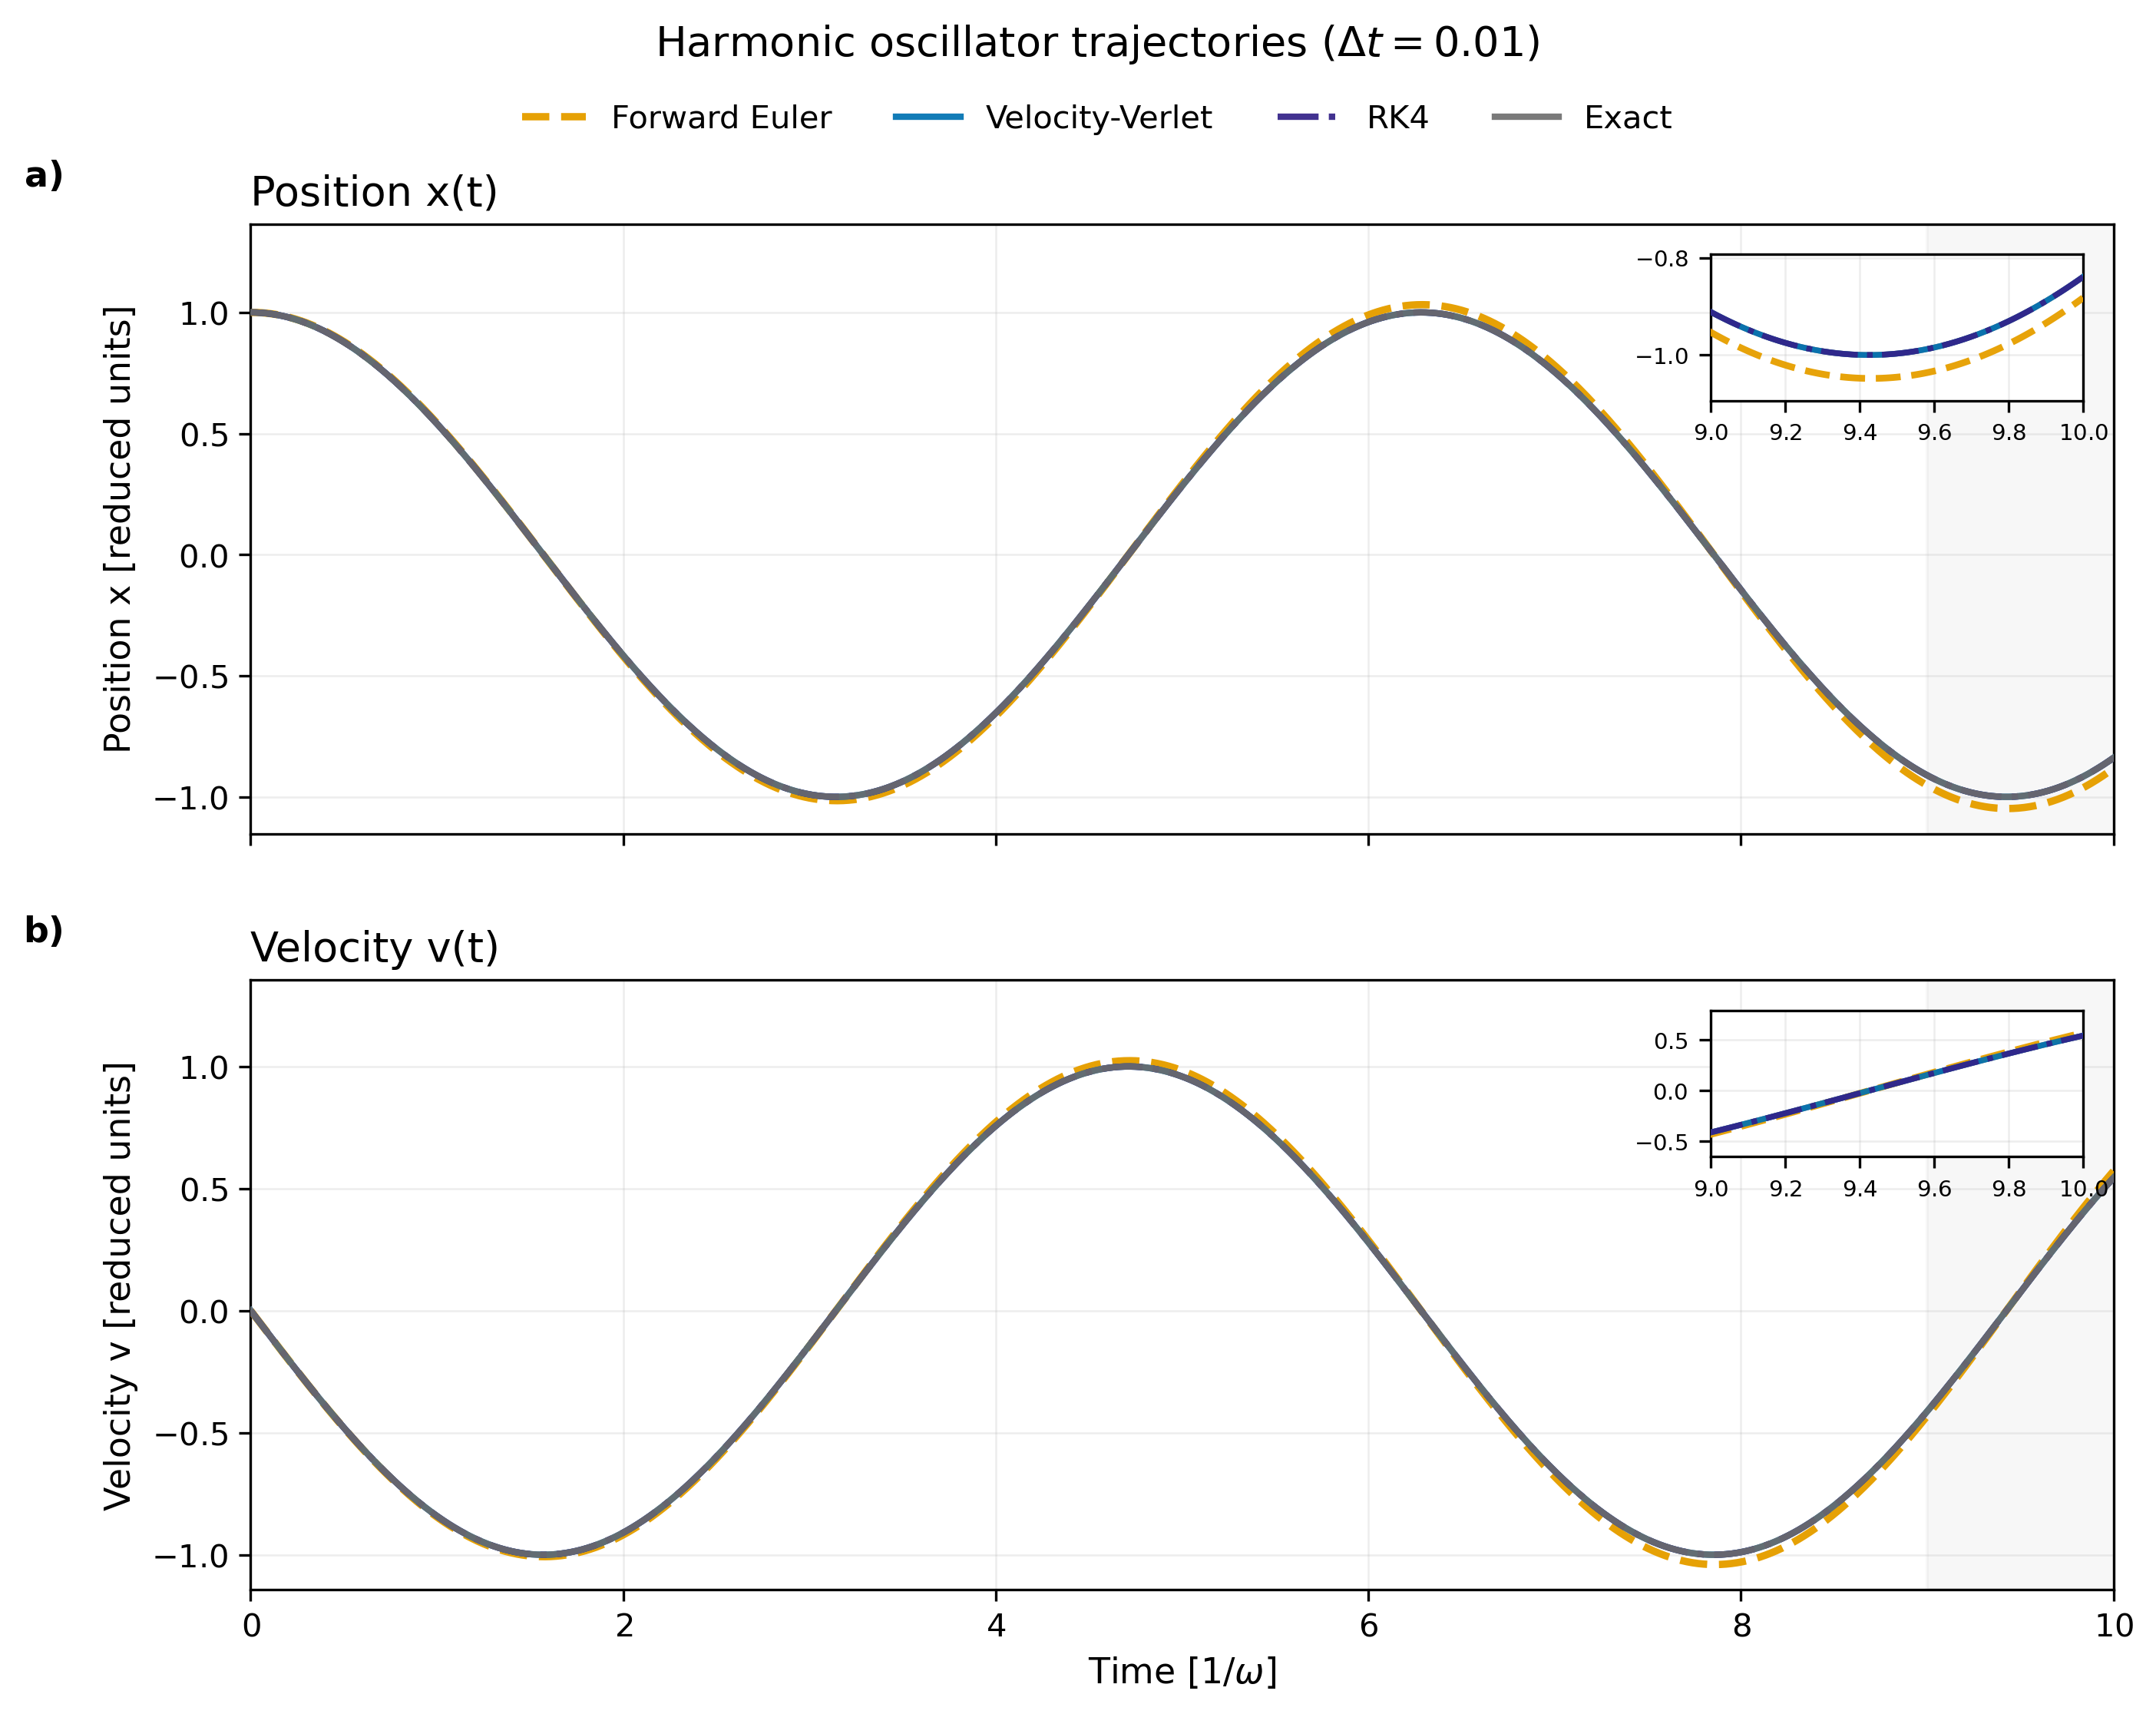
\includegraphics[width=0.575\textwidth]{results1_figure1ab_trajectories_dt0p01.png}%
  \hspace{0.005\textwidth}%
  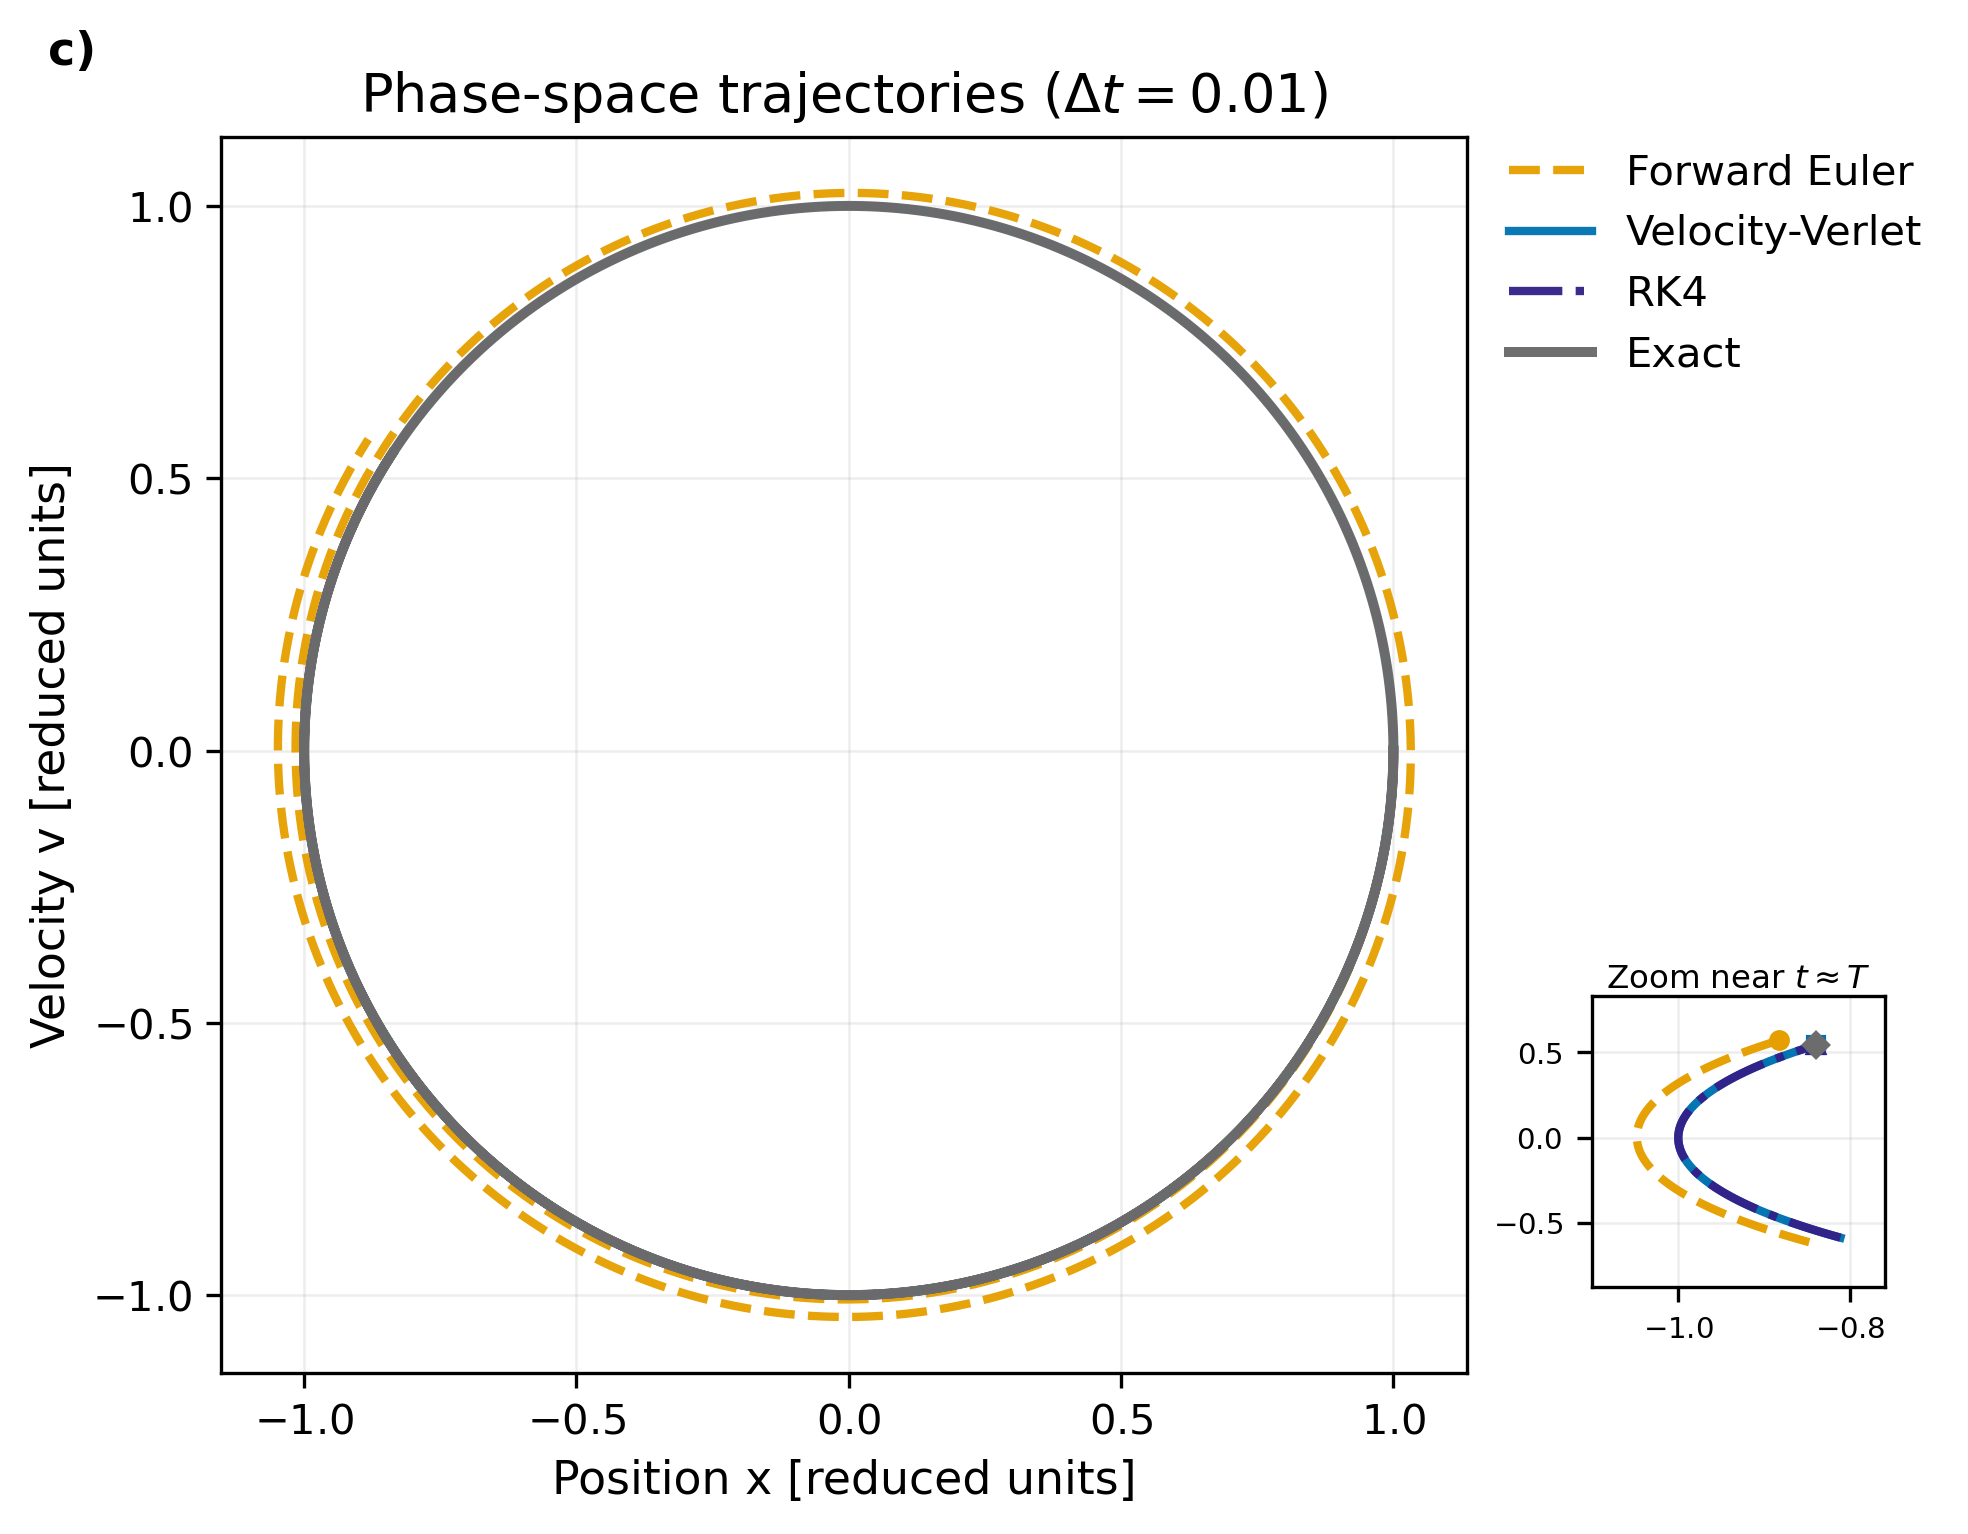
\includegraphics[width=0.405\textwidth]{results1_figure1c_phase_space_dt0p01.png}
  \caption{Harmonic oscillator trajectories and phase space at
    $\Delta t=0.01$, $\omega=1$, $T=10$.
    \textbf{(a)} Position $x(t)$ and \textbf{(b)} velocity $v(t)$: insets
    zoom to $t\in[9,10]$ where Euler (orange) exhibits visible phase lag;
    Velocity-Verlet (blue) and RK4 (dark blue) overlay the exact solution
    (grey).
    \textbf{(c)} Phase-space portrait: Euler spirals outward (non-symplectic,
    Liouville-violating); Velocity-Verlet returns a near-closed orbit
    (symplectic); RK4 is indistinguishable from exact.
    Inset: zoom near $t\approx T$ confirms the endpoint separation.}
  \label{fig:ho_traj}
\end{figure*}

\textbf{Sensitivity to timestep size.}
Figure~\ref{fig:ho_dtcomp} directly contrasts $\Delta t=0.01$ and
$\Delta t=0.5$.
At the coarse timestep, Forward Euler is numerically unstable (amplitude
grows to $|x|\approx 8$, spiralling outward);
Velocity-Verlet remains bounded despite poor accuracy---a key property of
symplectic integrators, which preserve qualitative dynamics even when
quantitative accuracy is degraded;
RK4 stays near the exact trajectory at both resolutions thanks to its
higher-order accuracy.

\begin{figure}[t]
  \centering
  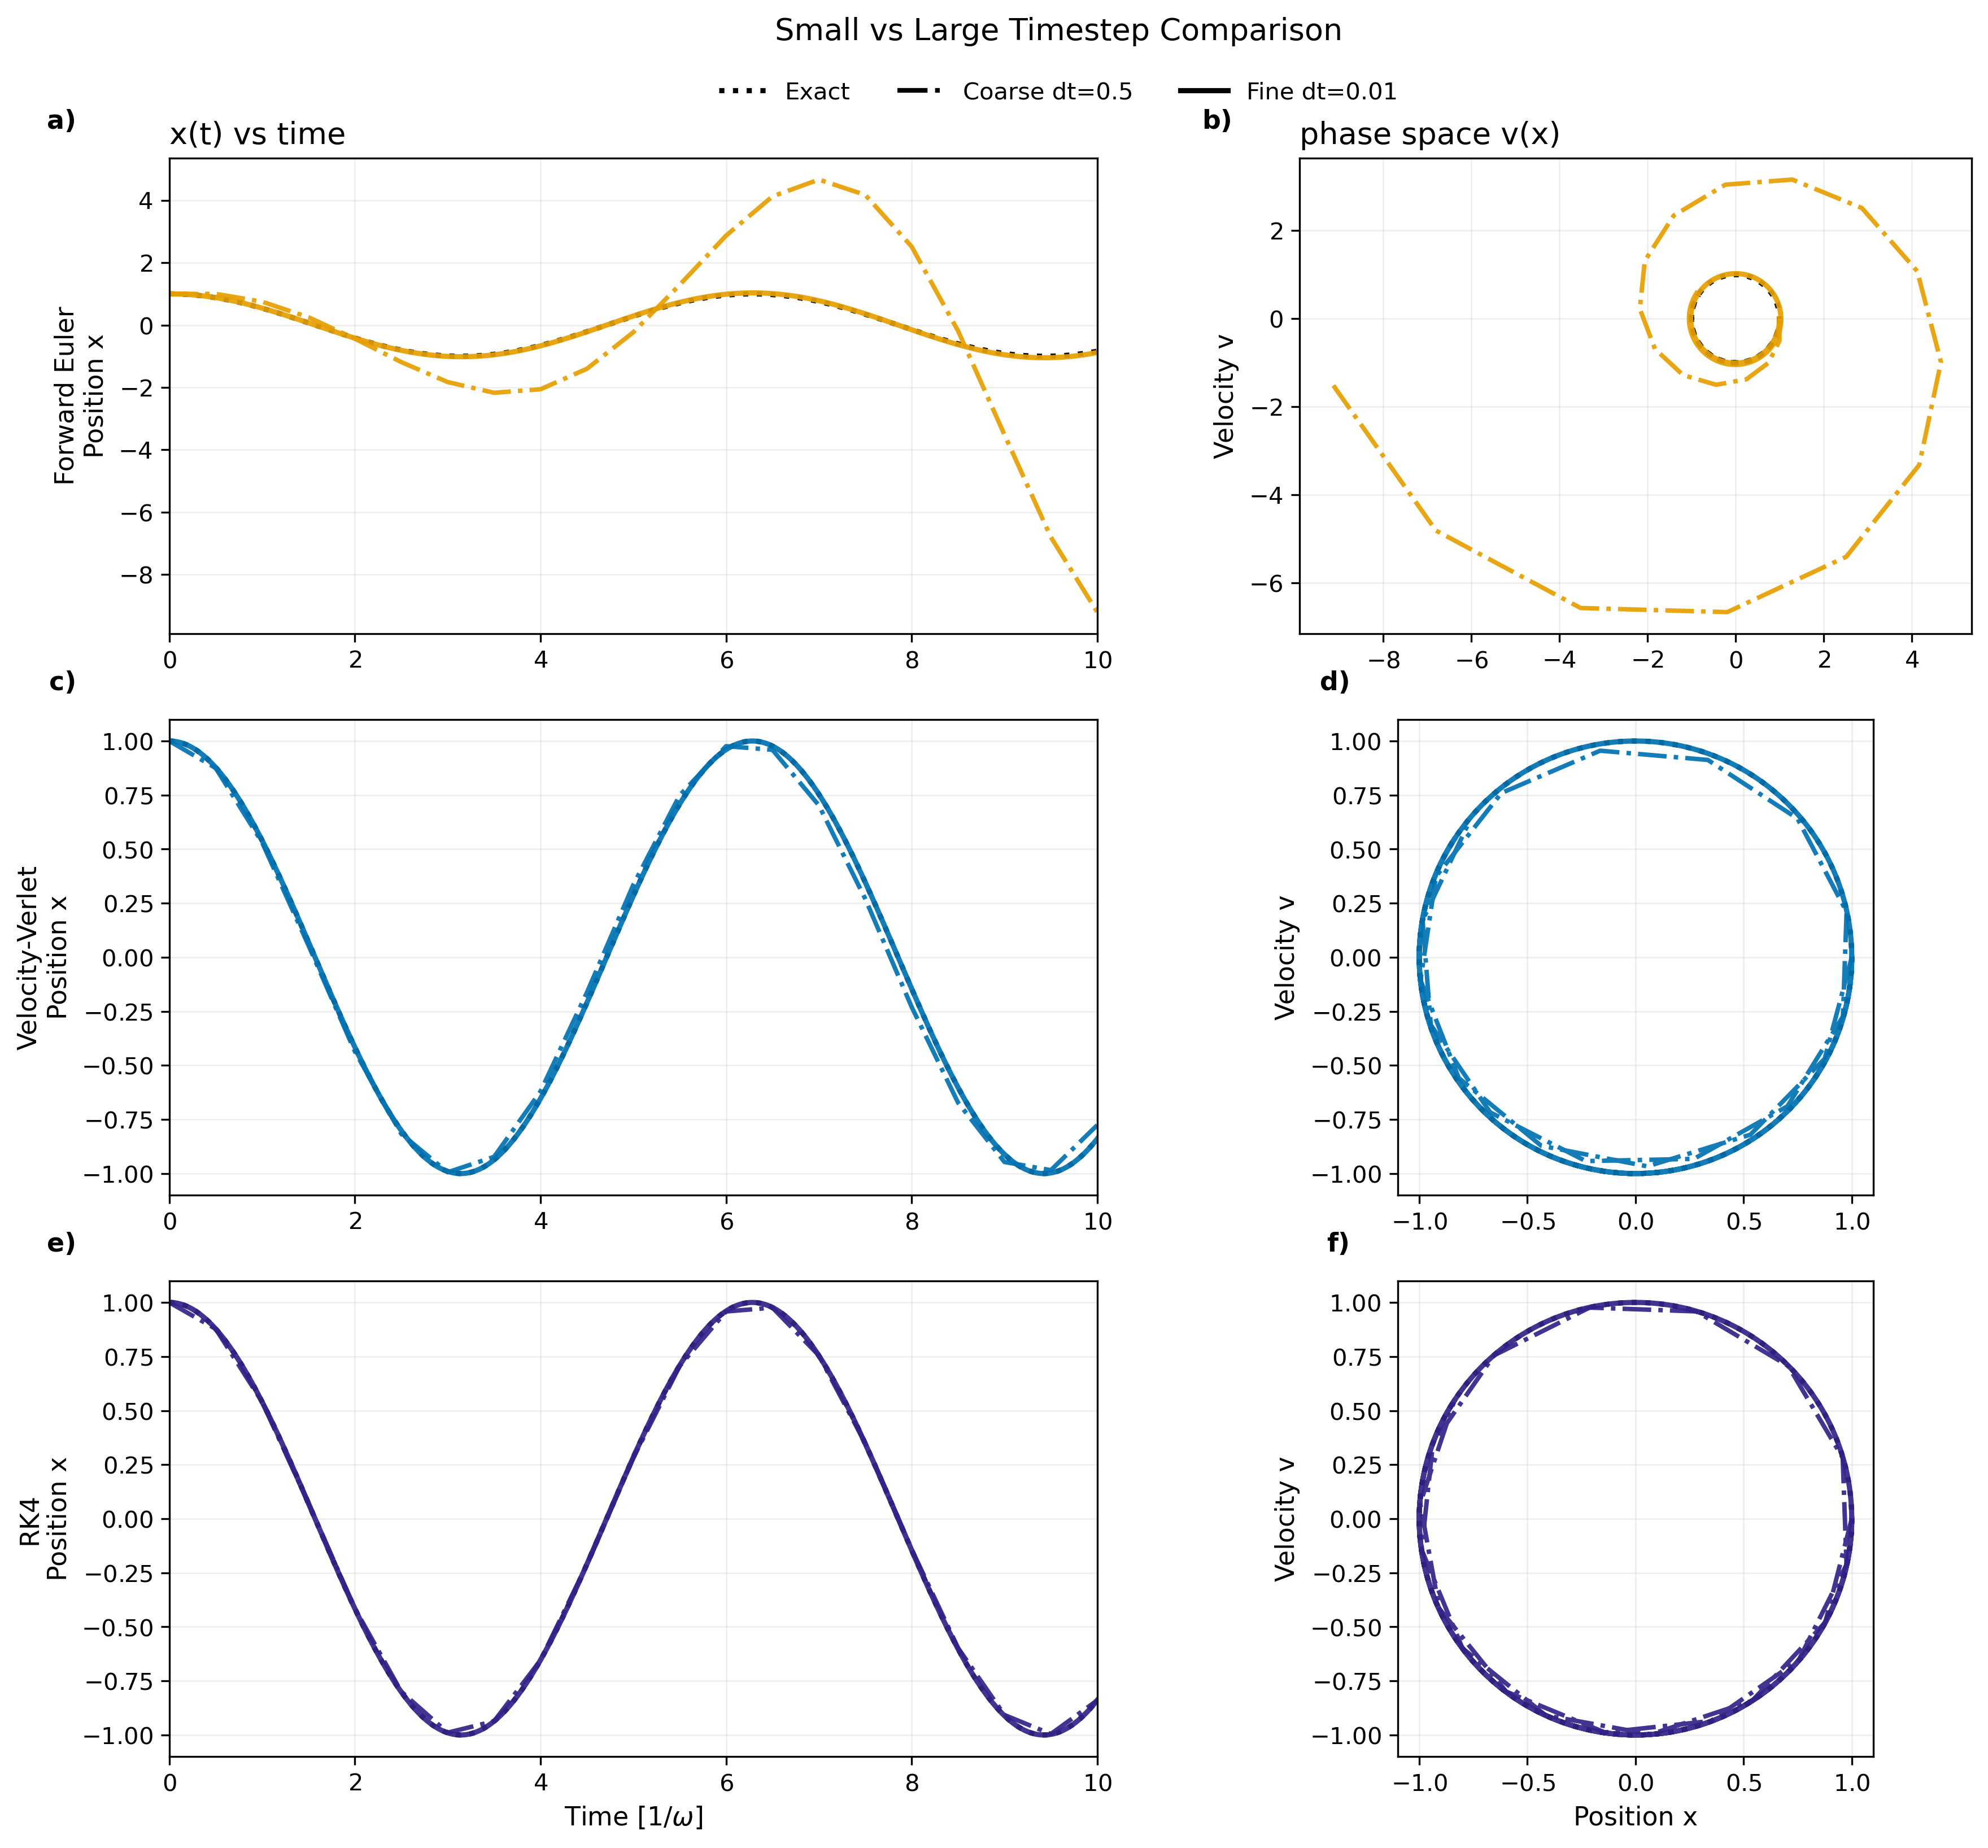
\includegraphics[width=\columnwidth]{results1_figure2_small_vs_large_dt.png}
  \caption{Effect of timestep on harmonic oscillator behaviour.
    \textbf{Left}: $x(t)$; \textbf{Right}: phase-space portrait.
    Each row shows $\Delta t=0.5$ (coarse, dash-dot) and $\Delta t=0.01$ (fine, solid).
    Euler (orange, top) is unstable at $\Delta t=0.5$;
    Velocity-Verlet (blue, centre) remains bounded even at the coarse timestep
    (symplectic structural stability);
    RK4 (dark blue, bottom) is accurate at both resolutions.}
  \label{fig:ho_dtcomp}
\end{figure}

\textbf{Convergence order.}
Figure~\ref{fig:ho_conv} presents the endpoint position error
$|x_{\rm num}(T{=}10)-\cos(10)|$ and RMS phase-space error as functions
of $\Delta t$ on log--log axes.
Table~\ref{tab:convergence} reports representative errors.
Linear regression over the asymptotic regime $\Delta t\le 0.1$ yields fitted
slopes of 1.05, 2.00, and 3.94 for Euler, Velocity-Verlet, and RK4,
confirming first-, second-, and fourth-order global convergence.
At $\Delta t=10^{-2}$, Velocity-Verlet is three orders of magnitude more
accurate than Euler; RK4 a further five.
RK4 saturates at ${\approx}3.6\times10^{-15}$ for
$\Delta t=5\times10^{-4}$, consistent with accumulation of IEEE~754
rounding errors over 20\,000 steps.

The $\mathcal{O}(\Delta t^2)$ global convergence of Velocity-Verlet reflects
accumulation over $T/\Delta t$ steps; the \emph{local} error per step is
$\mathcal{O}(\Delta t^4)$ due to symplectic cancellation of odd Taylor
terms---this local accuracy should not be conflated with fourth-order global
convergence.

\begin{table}[h]
  \centering
  \caption{Global position error at $T{=}10$ and fitted convergence slopes.
    RK4 $^\dagger$ denotes saturation at the IEEE~754 floor.}
  \label{tab:convergence}
  \small\setlength{\tabcolsep}{3.5pt}
  \begin{tabular}{@{}rccc@{}}
    \toprule
    $\Delta t$ & Euler & Vel.-Verlet & RK4 \\
    \midrule
    $10^{0}$   & $7.0\times10^{0}$   & $3.4\times10^{-1}$ & $2.2\times10^{-2}$ \\
    $10^{-1}$  & $2.3\times10^{-1}$  & $2.3\times10^{-3}$ & $3.9\times10^{-6}$ \\
    $10^{-2}$  & $2.0\times10^{-2}$  & $2.3\times10^{-5}$ & $4.5\times10^{-10}$ \\
    $10^{-3}$  & $2.0\times10^{-3}$  & $2.3\times10^{-7}$ & $5.3\times10^{-14}$ \\
    $5\!\times\!10^{-4}$ & $9.8\times10^{-4}$ & $5.7\times10^{-8}$ &
      $3.6\times10^{-15}$$^\dagger$ \\
    \midrule
    Slope & 1.05 & 2.00 & 3.94 \\
    \bottomrule
  \end{tabular}
\end{table}

\begin{figure*}[!t]
  \centering
  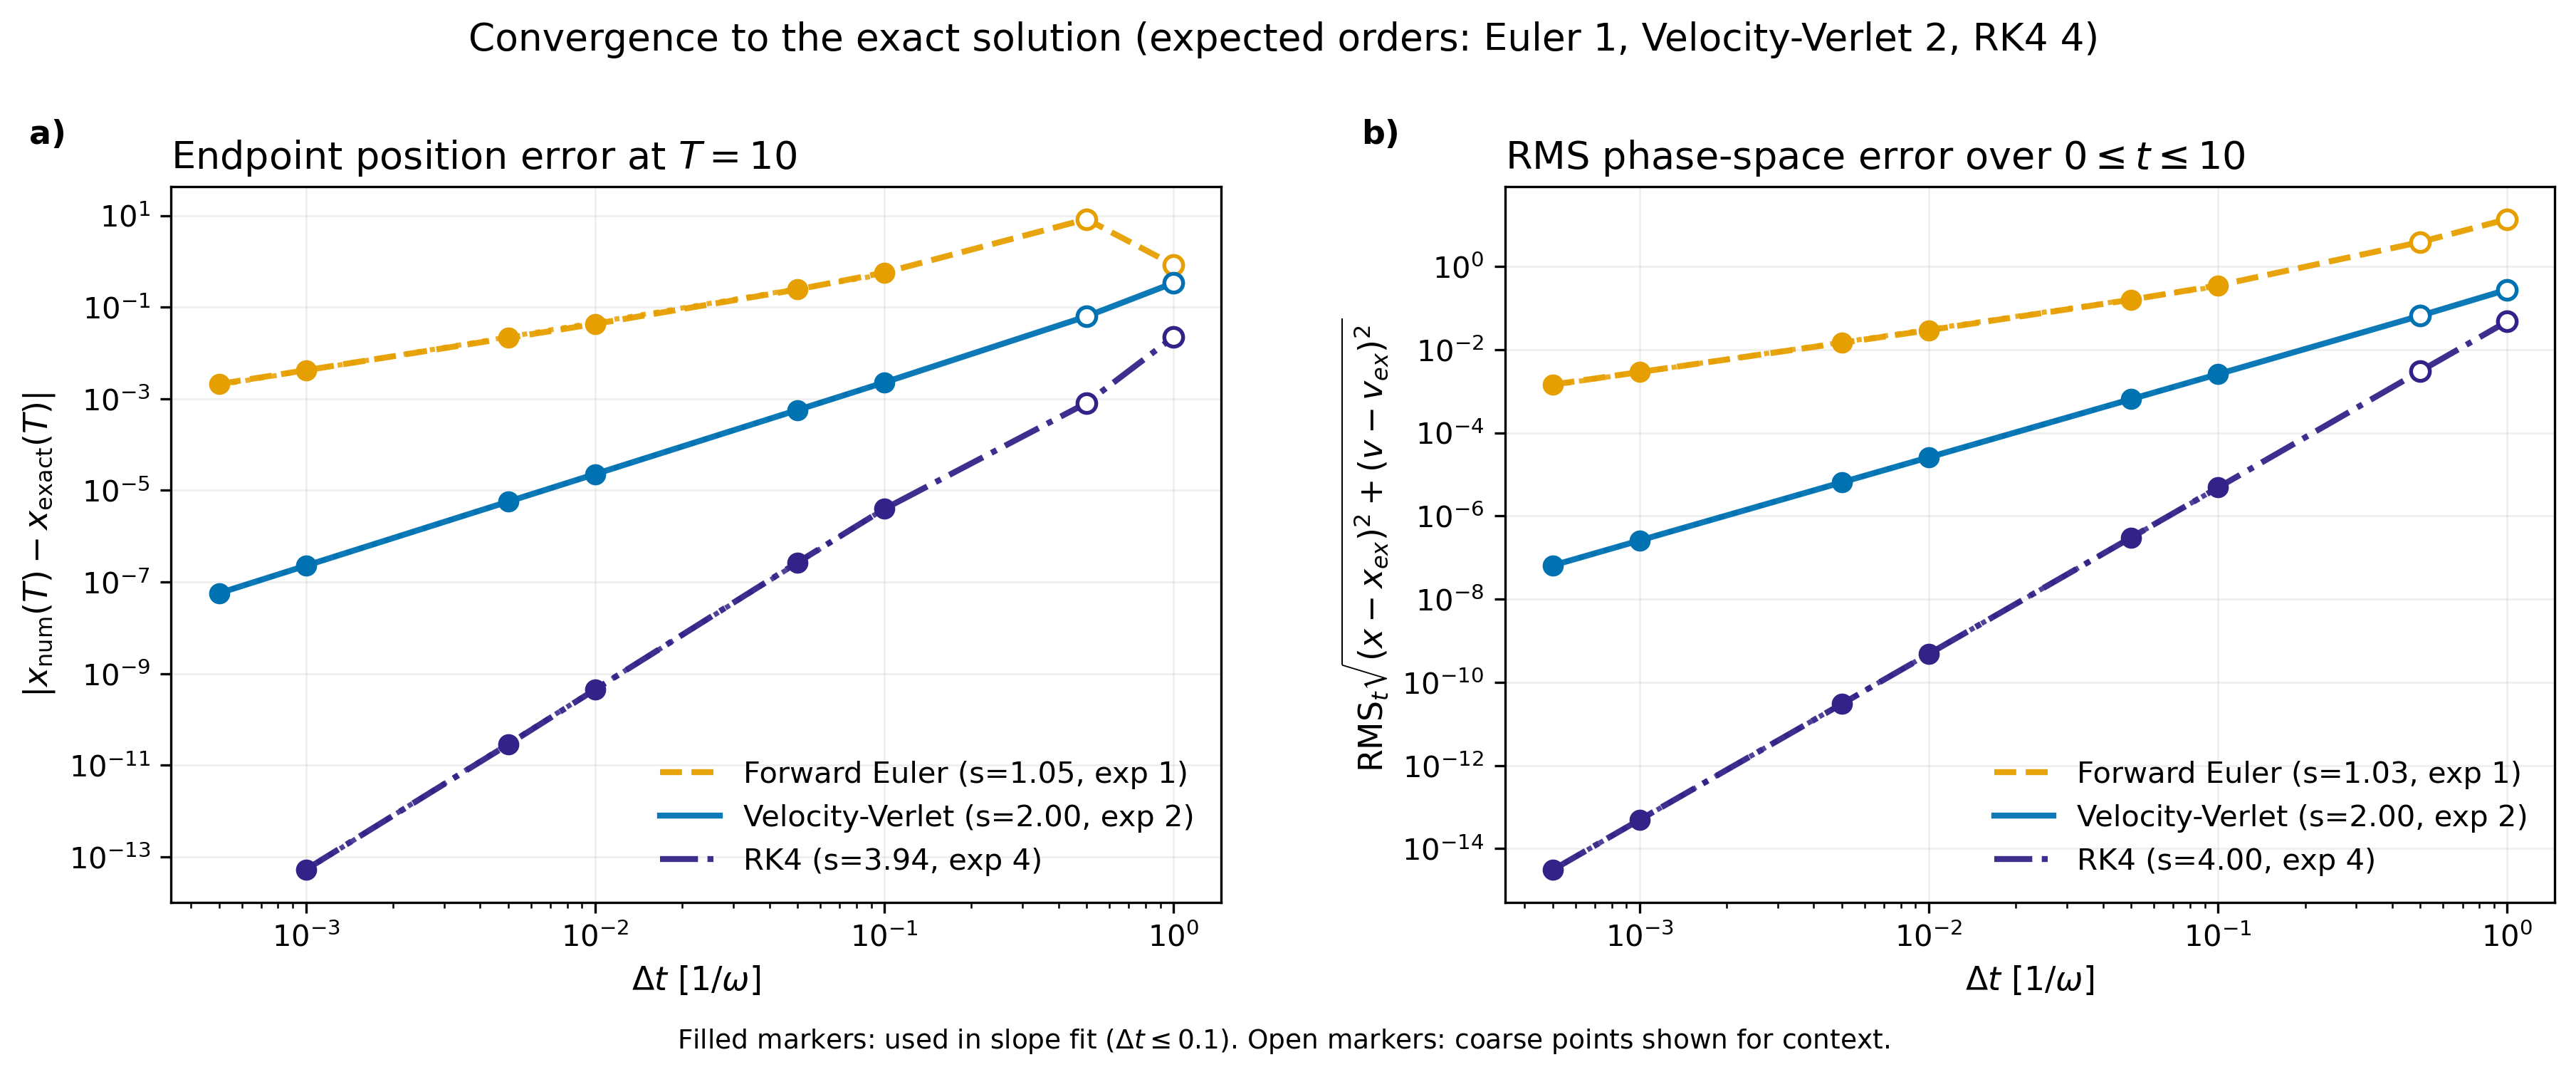
\includegraphics[width=0.96\textwidth]{results1_figure3_convergence_combined.png}
  \caption{Convergence of harmonic oscillator errors with timestep
    ($\omega=1$, $x_0=1$, $T=10$).
    \textbf{(a)} Endpoint position error; \textbf{(b)} RMS phase-space error.
    Filled markers: asymptotic fit domain ($\Delta t\le 0.1$); open: context only.
    Fitted slopes (Table~\ref{tab:convergence}) confirm orders 1.05, 2.00, 3.94.
    RK4 saturates at ${\approx}3.6\times10^{-15}$ (IEEE~754 floor, $\Delta t=5\times10^{-4}$).
    Reference lines (dashed) show exact integer slopes for comparison.}
  \label{fig:ho_conv}
\end{figure*}

\textbf{Energy conservation.}
Figure~\ref{fig:ho_energy} shows the relative energy deviation
$(E-E_0)/|E_0|$ at $\Delta t=0.01$.
Euler drifts monotonically to $10.5\%$ at $T=10$: a direct consequence
of non-symplectic phase-volume expansion.
Velocity-Verlet exhibits bounded oscillation at amplitude
${\approx}2.5\times10^{-5}$ (inset), confirming conservation of a shadow
Hamiltonian.
RK4 deviation is $1.4\times10^{-9}\%$ on this interval---negligible---but
its non-symplectic character would produce drift over much longer timescales.
This result directly illustrates the AMM Handout's core argument:
symplecticity governs long-time stability independently of truncation order.

\begin{figure}[ht]
  \centering
  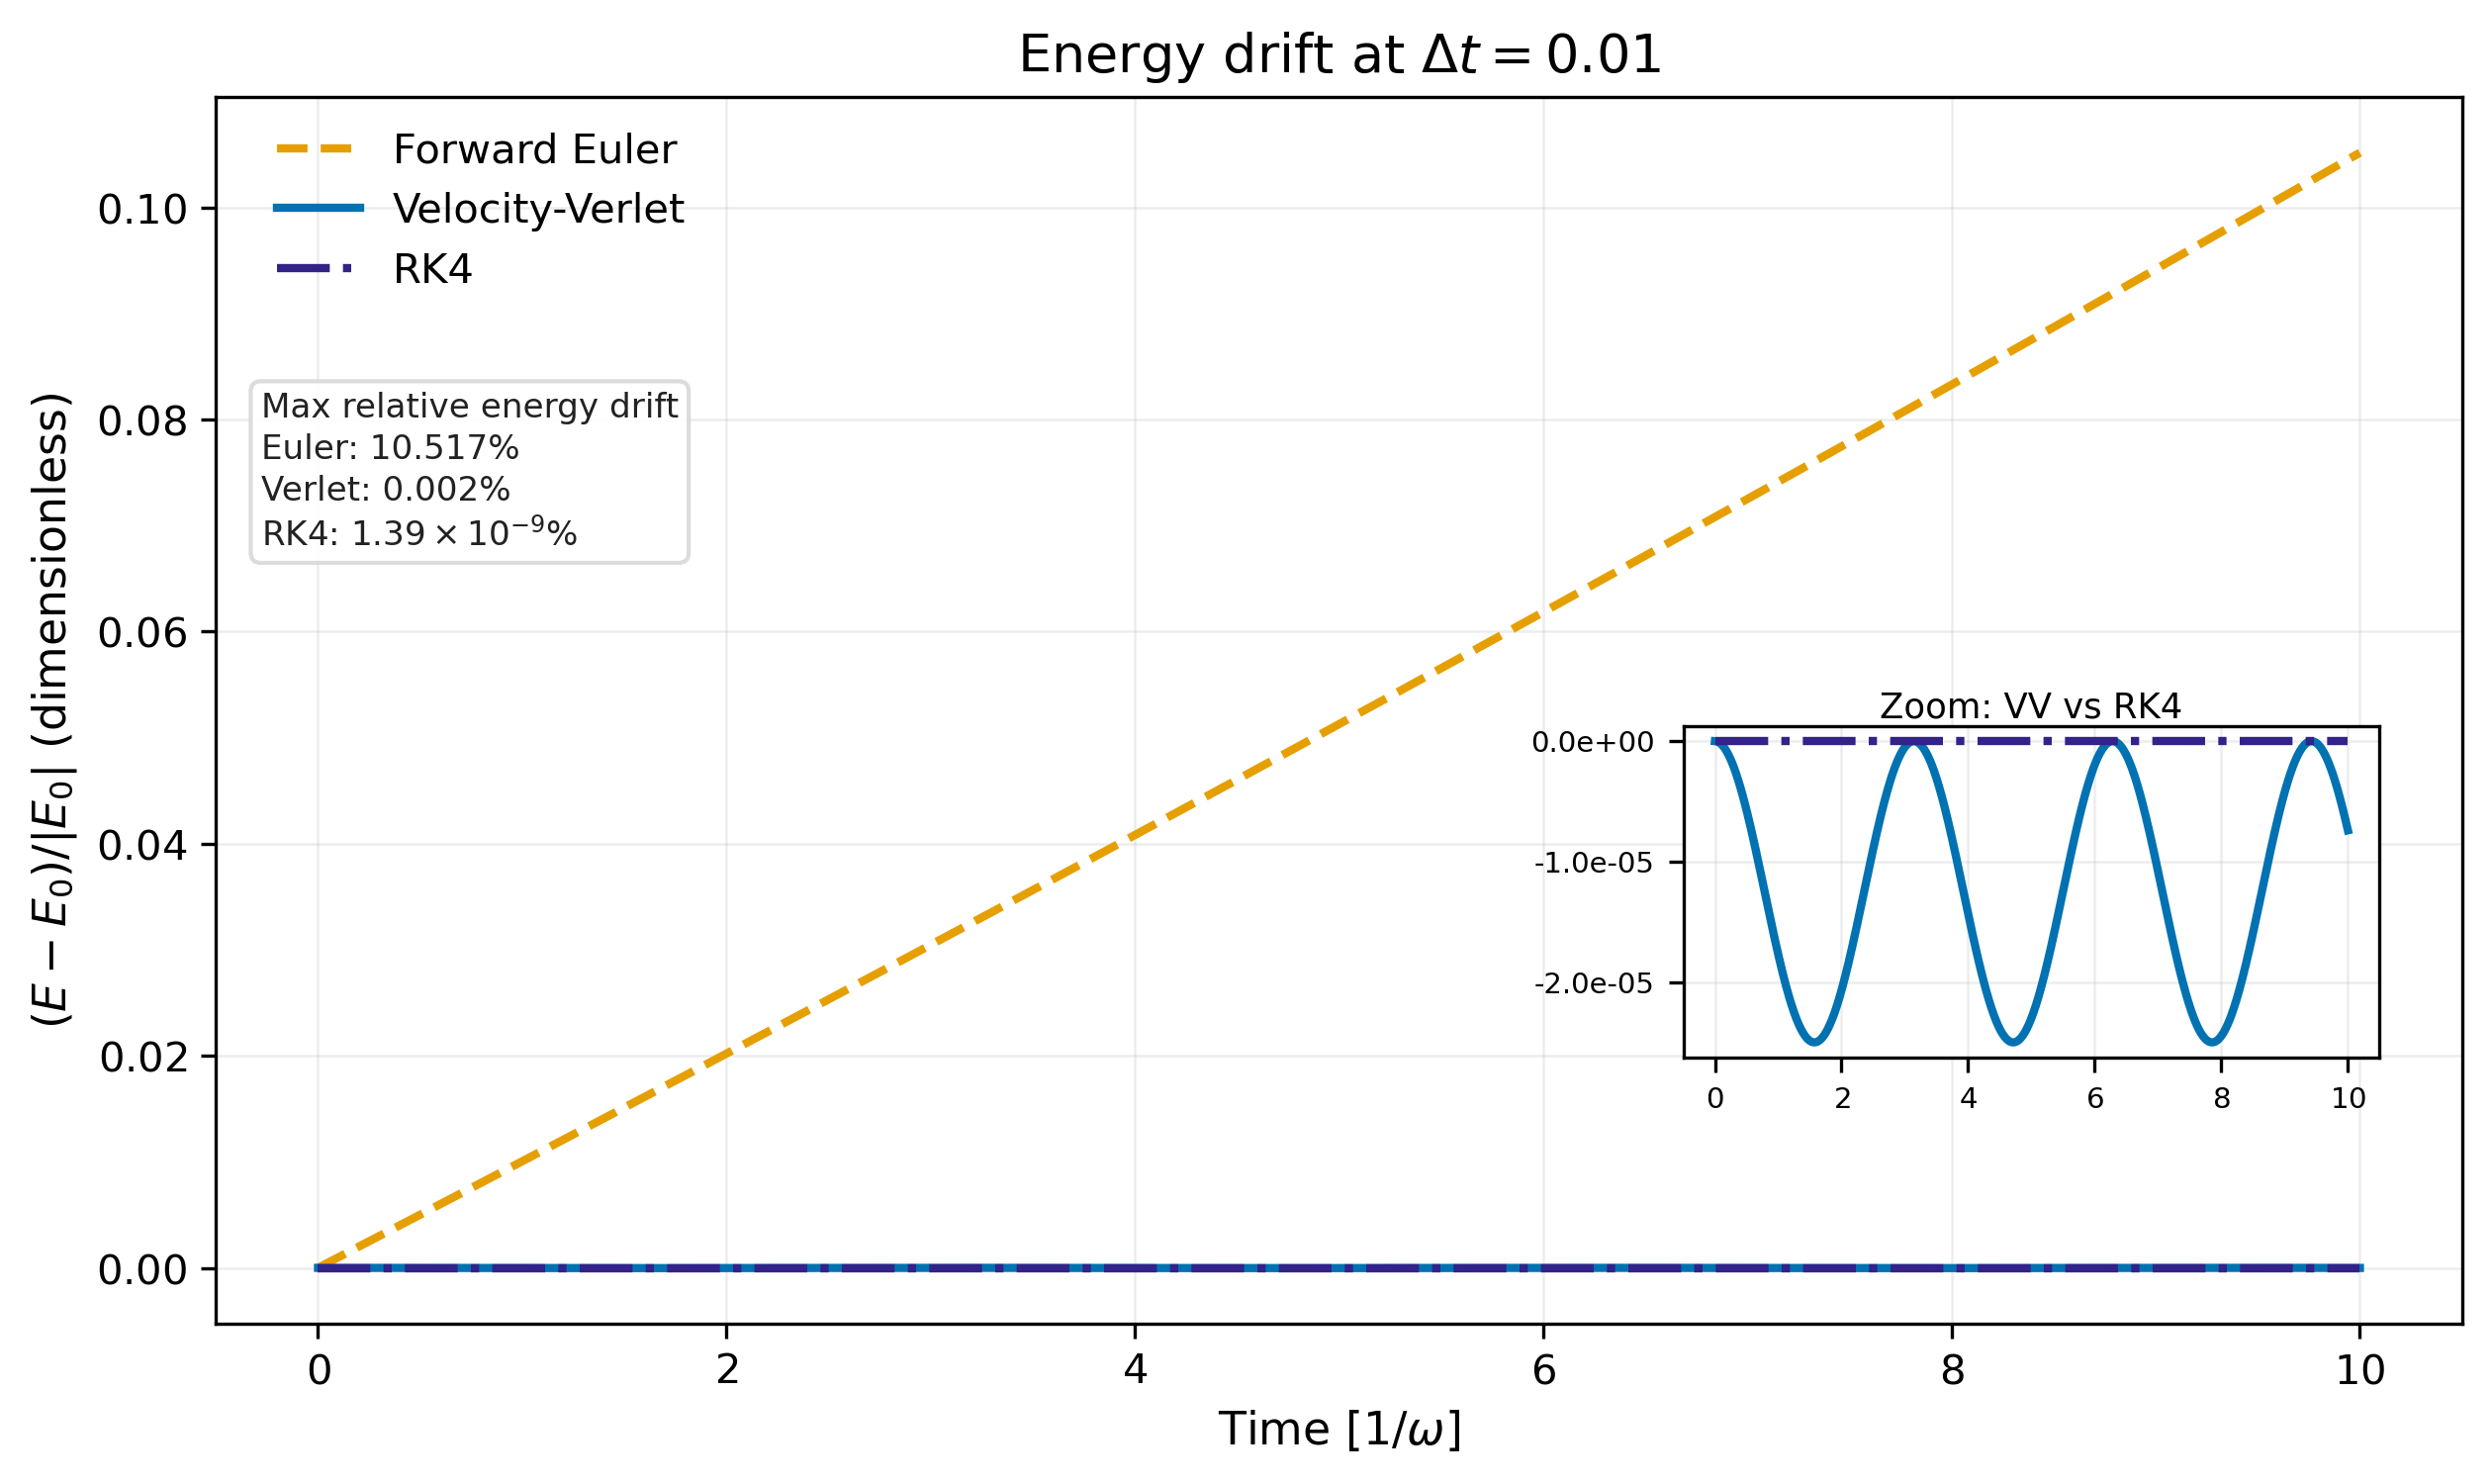
\includegraphics[width=\columnwidth]{results1_figure4_energy_diagnostic.png}
  \caption{Relative energy deviation $(E-E_0)/|E_0|$ for the harmonic
    oscillator ($\Delta t=0.01$, $T=10$).
    Euler (orange dashed) drifts linearly to 10.5\%; Velocity-Verlet (blue)
    is flat on the main panel.
    \textbf{Inset}: zoom reveals VV bounded oscillation at ${\approx}2.5\times10^{-5}$
    (shadow-Hamiltonian conservation) and negligible RK4 deviation
    ($1.4\times10^{-9}\%$).}
  \label{fig:ho_energy}
\end{figure}

\subsection{Lennard-Jones Argon Fluid}
\label{sec:lj_results}

The LJ argon system ($N=864$, $\Delta t=\SI{e-14}{s}$) is initialised on
an FCC lattice, equilibrated over 50 steps with velocity rescaling, and
then run for 100 NVE production steps at $P=4$ (1 ps total).
This constitutes the \emph{required production run} per the assignment brief.

\textbf{Energy conservation: required 100-step run.}
Figure~\ref{fig:lj_energy} shows the signed relative total-energy deviation
$\Delta E/E_0$ for both integrators over the 1~ps production window.
Velocity-Verlet (panel~a) maintains bounded deviation with
$\max|\Delta E/E_0|=0.082\%$ (mean $0.033\%$, final $+0.026\%$),
consistent with shadow-Hamiltonian conservation.
Forward Euler (panel~b) diverges to $+127.6\%$ within 1~ps, with the
deviation growing super-linearly as the unphysical energy injection
amplifies the forces.
The finite Velocity-Verlet deviations arise from three sources: (i)~the hard
cutoff at $r_c$ causes energy discontinuities when pairs cross the cutoff
radius; (ii)~residual force imbalances at the FCC-to-liquid relaxation
boundary generate local integration error; and (iii)~finite-timestep
truncation accumulates even under the shadow Hamiltonian.
A shifted-force cutoff---where both $V(r_c)=0$ and $\mathbf{F}(r_c)=\mathbf{0}$---would
eliminate contribution (i) and is standard in production codes.

\begin{figure}[t]
  \centering
  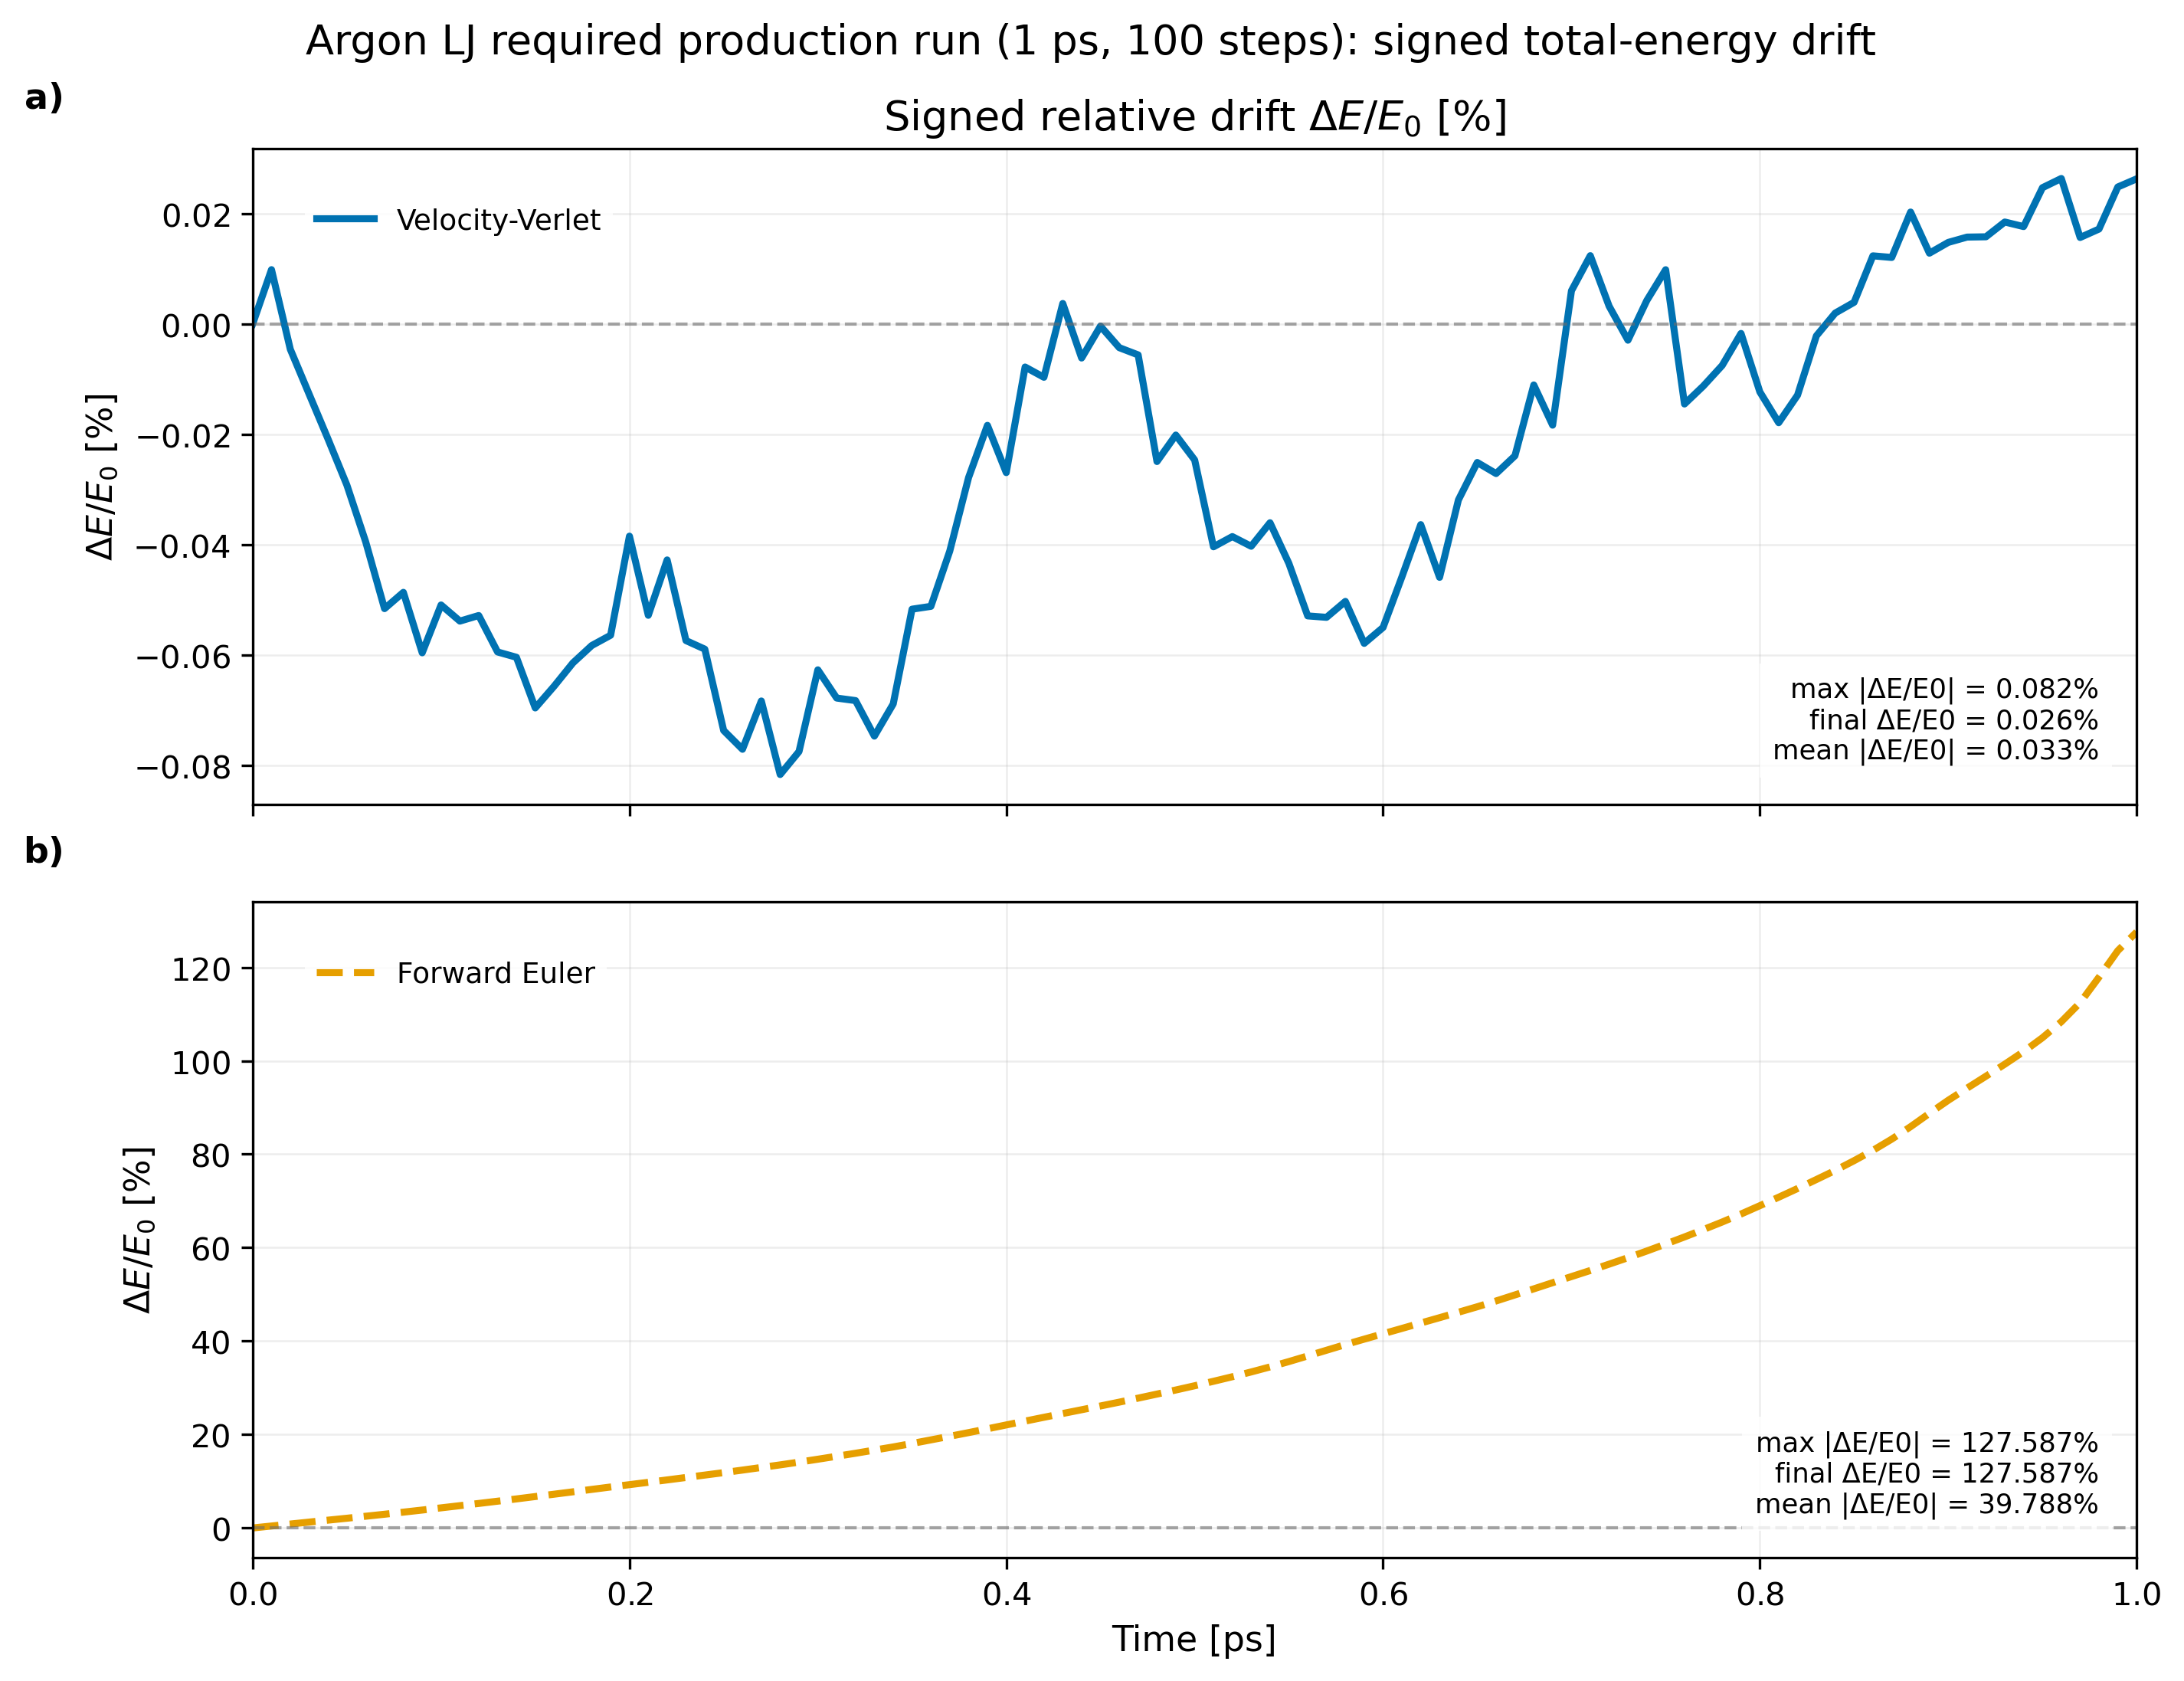
\includegraphics[width=\columnwidth]{results2_figure6_lj_brief_energy_100step_production.png}
  \caption{Signed relative total-energy deviation $\Delta E/E_0$ [\%]
    during the required 100-step ($\Delta t=\SI{e-14}{s}$) NVE production run
    for LJ argon ($N=864$, $P=4$, equilibrated to $T=\SI{94.4}{K}$).
    \textbf{(a)} Velocity-Verlet: bounded oscillation, $\max|\Delta E/E_0|=0.082\%$,
    mean $0.033\%$.
    \textbf{(b)} Forward Euler: monotonic divergence to $+127.6\%$, demonstrating
    catastrophic non-symplectic energy injection.}
  \label{fig:lj_energy}
\end{figure}

\textbf{Temperature.}
Figure~\ref{fig:lj_temp} shows the corresponding temperature evolution.
Velocity-Verlet holds $T = (94.4\pm1.4)\,\si{K}$ over the full production
window (mean $94.42\,\si{K}$), consistent with NVE conservation.
Forward Euler heats exponentially from $\SI{94.4}{K}$ to
${\sim}\SI{400}{K}$ within 1~ps (mean $\SI{185}{K}$);
this temperature runaway is the direct thermodynamic signature of Euler's
non-symplectic energy injection and confirms its unsuitability for production
MD even from a well-equilibrated starting configuration.

\begin{figure}[ht]
  \centering
  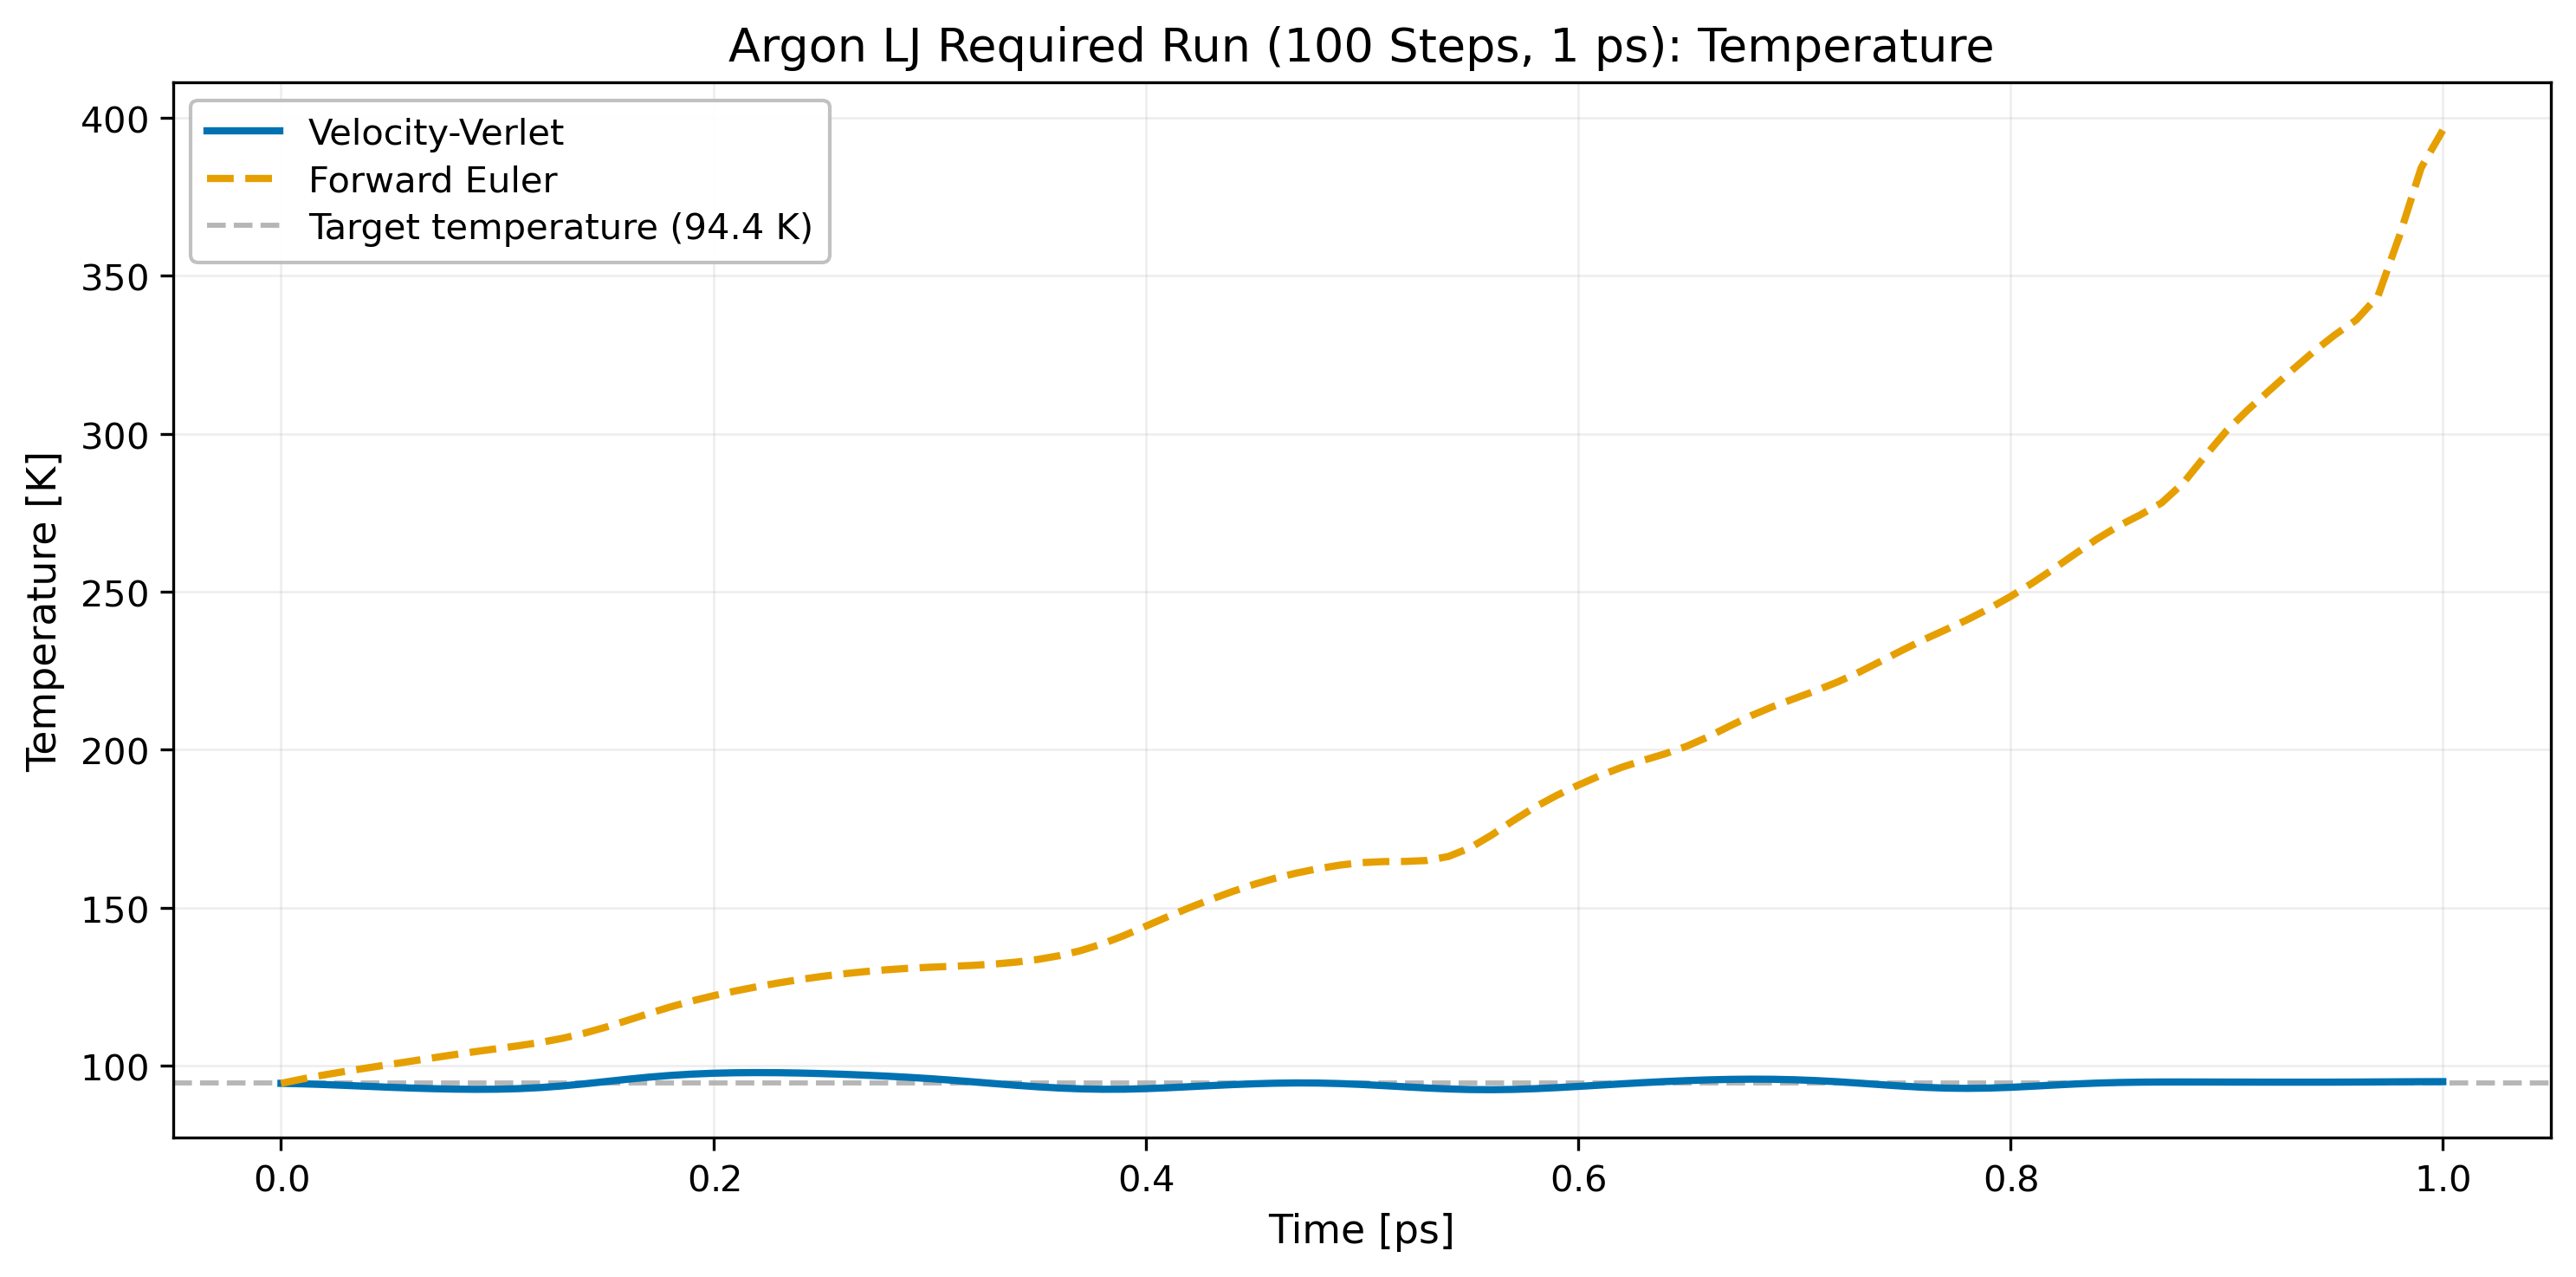
\includegraphics[width=\columnwidth]{results2_figure7_lj_brief_temperature_100step_production.png}
  \caption{Instantaneous temperature during the required 100-step NVE production
    run ($N=864$, $\Delta t=\SI{e-14}{s}$).
    Velocity-Verlet (blue) holds $T\approx\SI{94.4}{K}$ (grey dashed);
    Forward Euler (orange) heats to ${\sim}\SI{400}{K}$ by 1~ps,
    directly reflecting the energy drift of Fig.~\ref{fig:lj_energy}.}
  \label{fig:lj_temp}
\end{figure}

\textbf{Radial distribution function.}
To further validate the simulated liquid structure, a separate extended run
was performed (20\,000 NVE steps at $P=4$, $g(r)$ accumulated after a
200-step discard and sampled every 5 steps).
Figure~\ref{fig:lj_rdf} shows $g(r)$ alongside a reference guide digitised
from Fig.~2 of~\citet{Rahman1964}.
The first peak at $r/\sigma\approx1.09$ ($g\approx2.84$), first minimum at
$r/\sigma\approx1.55$, second peak at $r/\sigma\approx2.07$ ($g\approx1.25$),
and long-range tail ($\langle g\rangle=1.002$ for $r>4\sigma$) all compare
favourably with Rahman's published liquid-structure data.
This comparison is \emph{qualitative to semi-quantitative}: the Rahman
reference was constructed from manually anchored digitisation points, and
exact reproduction is not expected given different initial configurations
and finite run length.
Note that the required 100-step run (1~ps) is insufficient for $g(r)$
accumulation; the RDF presented here derives from this separate extended run,
included as additional structural validation.

\begin{figure}[h]
  \centering
  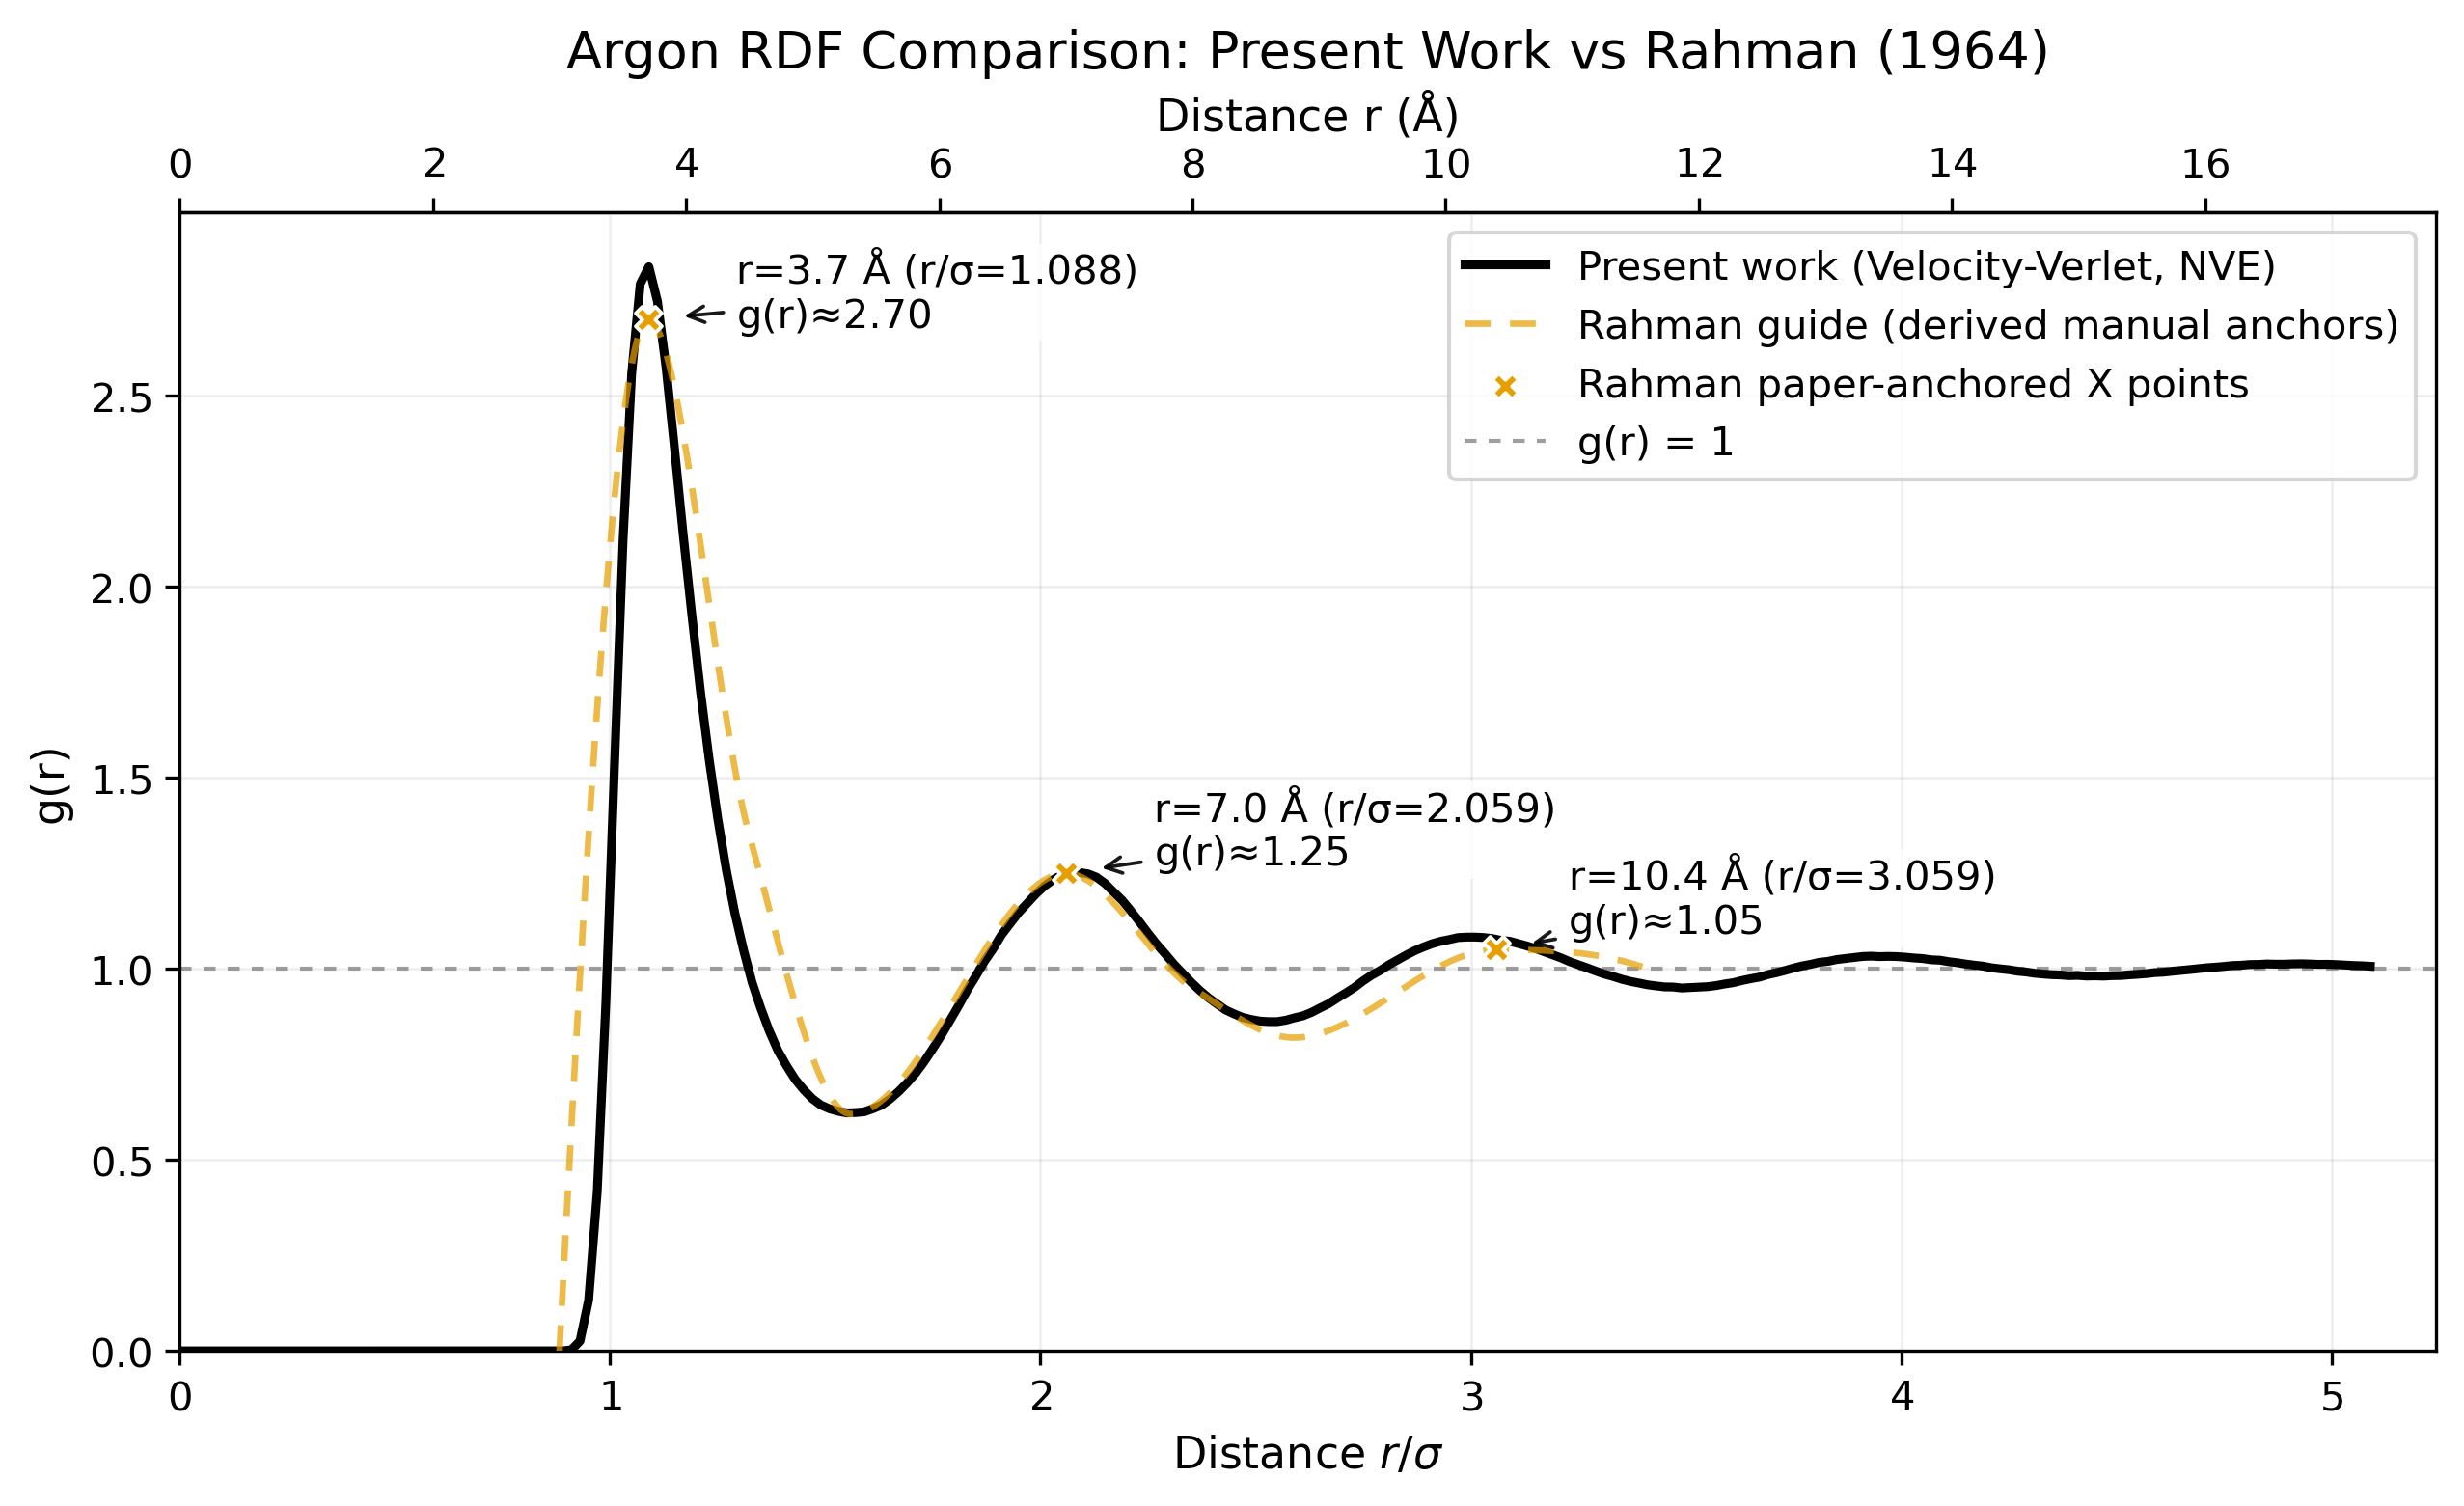
\includegraphics[width=\columnwidth]{results2_figure8_lj_rdf_comparison_rahman1964.png}
  \caption{Radial distribution function $g(r)$ from an extended 20\,000-step
    NVE run (Velocity-Verlet, $N=864$, $P=4$; $g(r)$ sampled every 5 steps
    after a 200-step discard).
    Blue: present work; orange dashed: reference guide from~\citet{Rahman1964}
    (digitised, manually anchored).
    First peak: $r/\sigma\approx1.09$, $g\approx2.84$; second peak:
    $r/\sigma\approx2.07$, $g\approx1.25$; tail $\langle g\rangle=1.002\to1$.
    The comparison is qualitative to semi-quantitative; exact reproduction
    is not claimed.}
  \label{fig:lj_rdf}
\end{figure}

\subsection{Parallel Scaling Analysis}
\label{sec:scaling}

All scaling runs use Velocity-Verlet, 100 steps, fixed seed,
$\Delta t=\SI{e-14}{s}$, and no file output.
Wall time is the maximum across ranks (\texttt{MPI\_Reduce(MPI\_MAX)});
communication time is the maximum \texttt{MPI\_Allgatherv} wall time
accumulated per rank.

\subsubsection*{Strong scaling}

\begin{table}[ht]
  \centering
  \caption{Strong scaling results ($N=2048$, 100 steps).
    Wall and communication times in seconds.}
  \label{tab:strong}
  \small\setlength{\tabcolsep}{3pt}
  \begin{tabular}{@{}rrrrrr@{}}
    \toprule
    $P$ & $T_{\rm wall}$ [s] & $T_{\rm comm}$ [s] & Comm\,\% & $S(P)$ & $E(P)$ \\
    \midrule
     1 & 45.96 & 0.001 &  0.0 &  1.00 & 1.000 \\
     2 & 23.15 & 0.244 &  1.1 &  1.99 & 0.993 \\
     4 & 12.00 & 0.661 &  5.5 &  3.83 & 0.957 \\
     8 &  6.09 & 0.554 &  9.1 &  7.55 & 0.944 \\
    16 &  3.21 & 0.367 & 11.4 & 14.30 & 0.894 \\
    24 &  2.37 & 0.319 & 13.5 & 19.42 & 0.809 \\
    32 &  1.91 & 0.290 & 15.2 & 24.12 & 0.754 \\
    \bottomrule
  \end{tabular}
\end{table}

Table~\ref{tab:strong} and Figure~\ref{fig:strong} show speedup
$S(P)=T_1/T_P$ and efficiency $E(P)=S(P)/P$ at fixed $N=2048$.
Scaling is near-ideal up to $P=8$ (efficiency $>94\%$), demonstrating that
the $\mathcal{O}(N^2/P)$ force computation dominates and \texttt{MPI\_Allgatherv}
overhead is small in this regime.

Beyond $P=8$, efficiency falls progressively: at $P=32$, $S(32)=24.1\times$
with $E=75\%$ and communication accounts for $15.2\%$ of wall time.
Amdahl's law~\citep{Amdahl1967},
\begin{equation}
  S(P) = \frac{1}{f + (1-f)/P}, \label{eq:amdahl}
\end{equation}
fitted via nonlinear least-squares over all $P>1$ yields $f\approx0.010$.
This is an \emph{empirical descriptor} of the measured curve, not a literal
hardware-independent serial fraction: Eq.~\eqref{eq:amdahl} assumes constant
$f$ and negligible communication, but the \texttt{MPI\_Allgatherv} overhead
grows monotonically with $P$ (Table~\ref{tab:strong}, 1.1\% at $P=2$ to
15.2\% at $P=32$), so the fit underestimates the true bottleneck at high $P$.
The Amdahl fit slightly overestimates the measured speedup at $P\ge 24$,
as expected.

\begin{figure*}[!t]
  \centering
  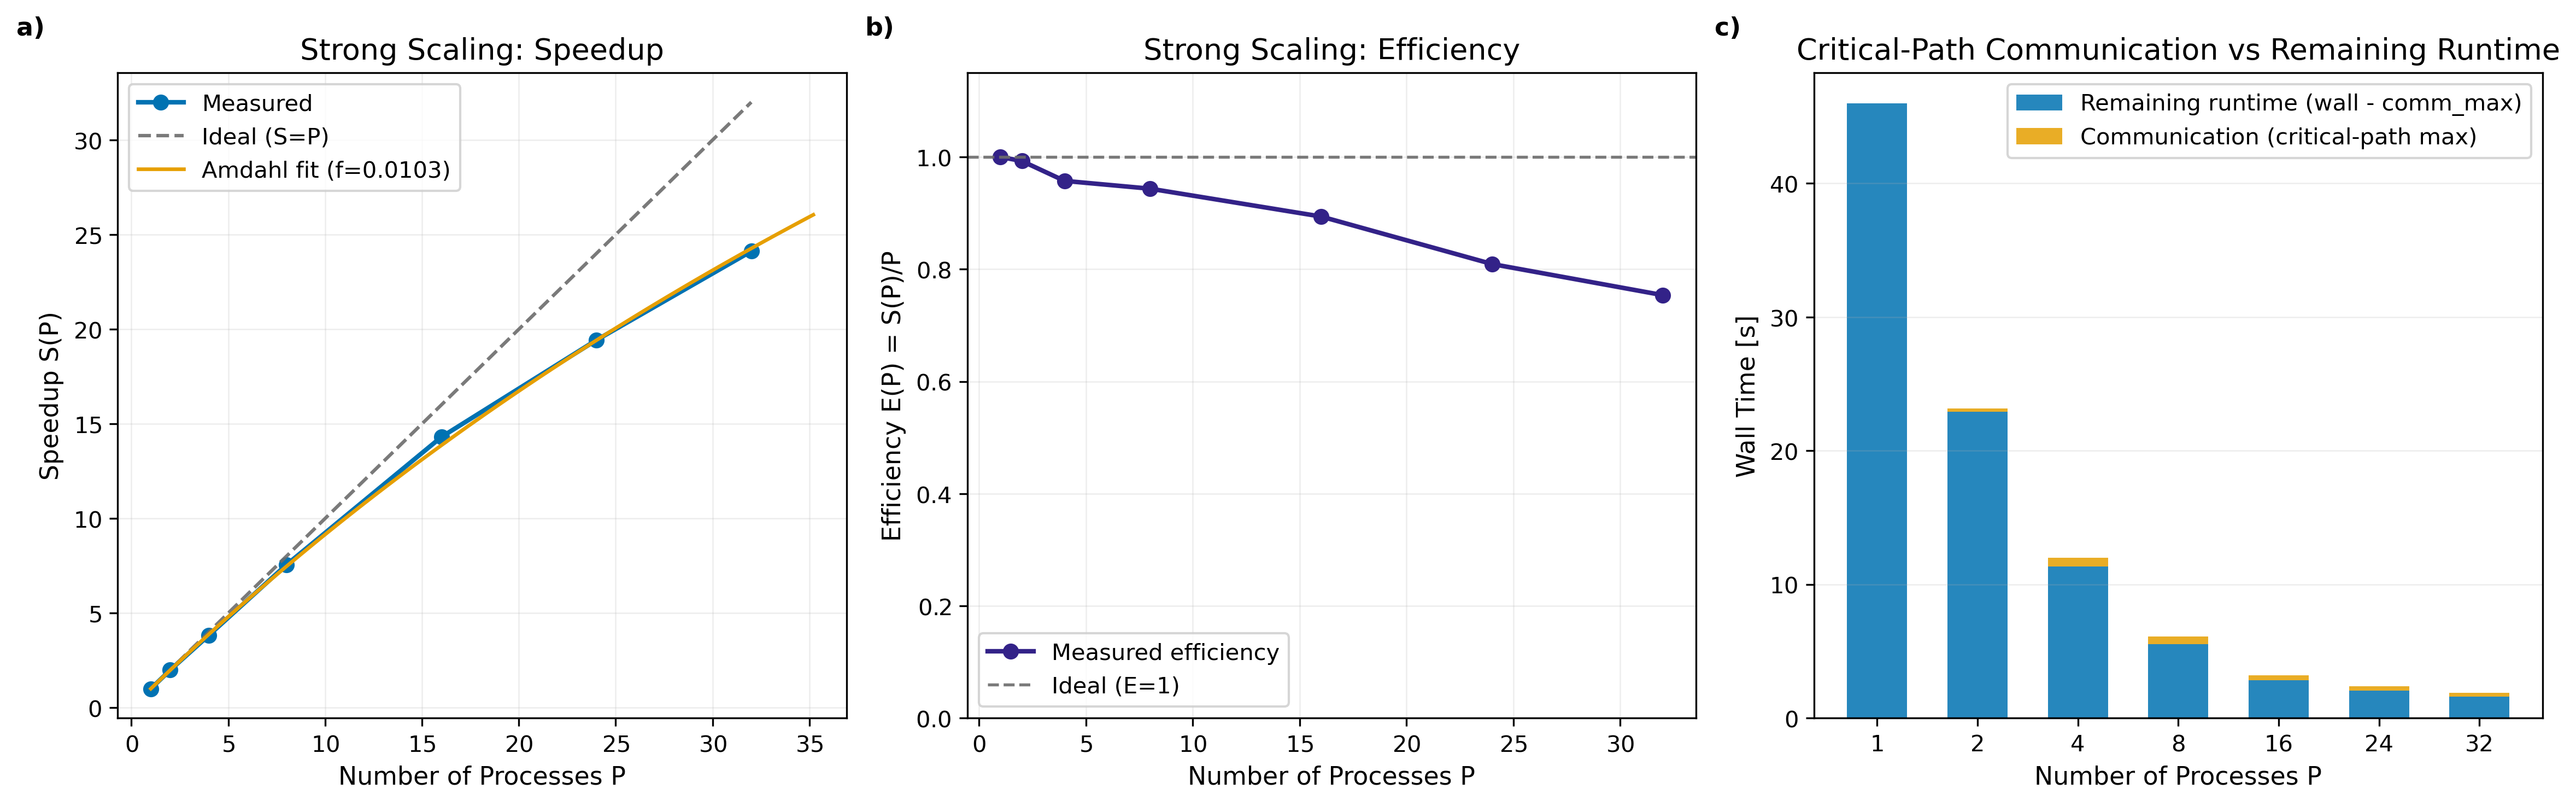
\includegraphics[width=0.96\textwidth]{results3_figure10abc_strong_scaling_speedup_efficiency_breakdown.png}
  \caption{Strong scaling ($N=2048$ fixed, Velocity-Verlet, 100 steps,
    dual-socket Intel Xeon Silver 4314 node).
    \textbf{(a)} Speedup $S(P)$: ideal line (grey dashed) and Amdahl fit
    (Eq.~\ref{eq:amdahl}, $f=0.010$, orange). Near-ideal to $P=8$; $S(32)=24.1\times$.
    \textbf{(b)} Parallel efficiency $E(P)$: above 94\% for $P\le 8$, dropping to 75\%
    at $P=32$.
    \textbf{(c)} Critical-path communication (orange) vs.\ remaining wall time (blue):
    communication fraction grows from $0\%$ to $15\%$, explaining the Amdahl
    fit deviation at high $P$.}
  \label{fig:strong}
\end{figure*}

\subsubsection*{Size scaling}

Figure~\ref{fig:size} shows wall time and its components at fixed $P=16$
for $N\in\{108, 256, 500, 864, 1372, 2048\}$.
Power-law fits over $N\ge500$ yield wall time $\propto N^{1.85}$ and
compute-only time (wall minus max-rank communication) $\propto N^{1.93}$,
approaching the expected $\mathcal{O}(N^2)$ asymptote.
The sub-quadratic wall-time exponent is consistent with the $\mathcal{O}(N)$
\texttt{MPI\_Allgatherv} communication contributing a sub-dominant term;
excluding it brings the exponent to $1.93$, which is close to the
theoretical value.
Small-$N$ points ($N=108$, 256) are excluded from the power-law fit:
the communication fraction is 51\% at $N=108$ and 27\% at $N=256$,
so these points do not reflect the asymptotic compute-dominated regime.
By $N=2048$ the communication fraction has fallen to $13\%$ (Fig.~\ref{fig:size}b),
confirming that the $\mathcal{O}(N^2)$ force loop increasingly dominates.

\begin{figure*}[!t]
  \centering
  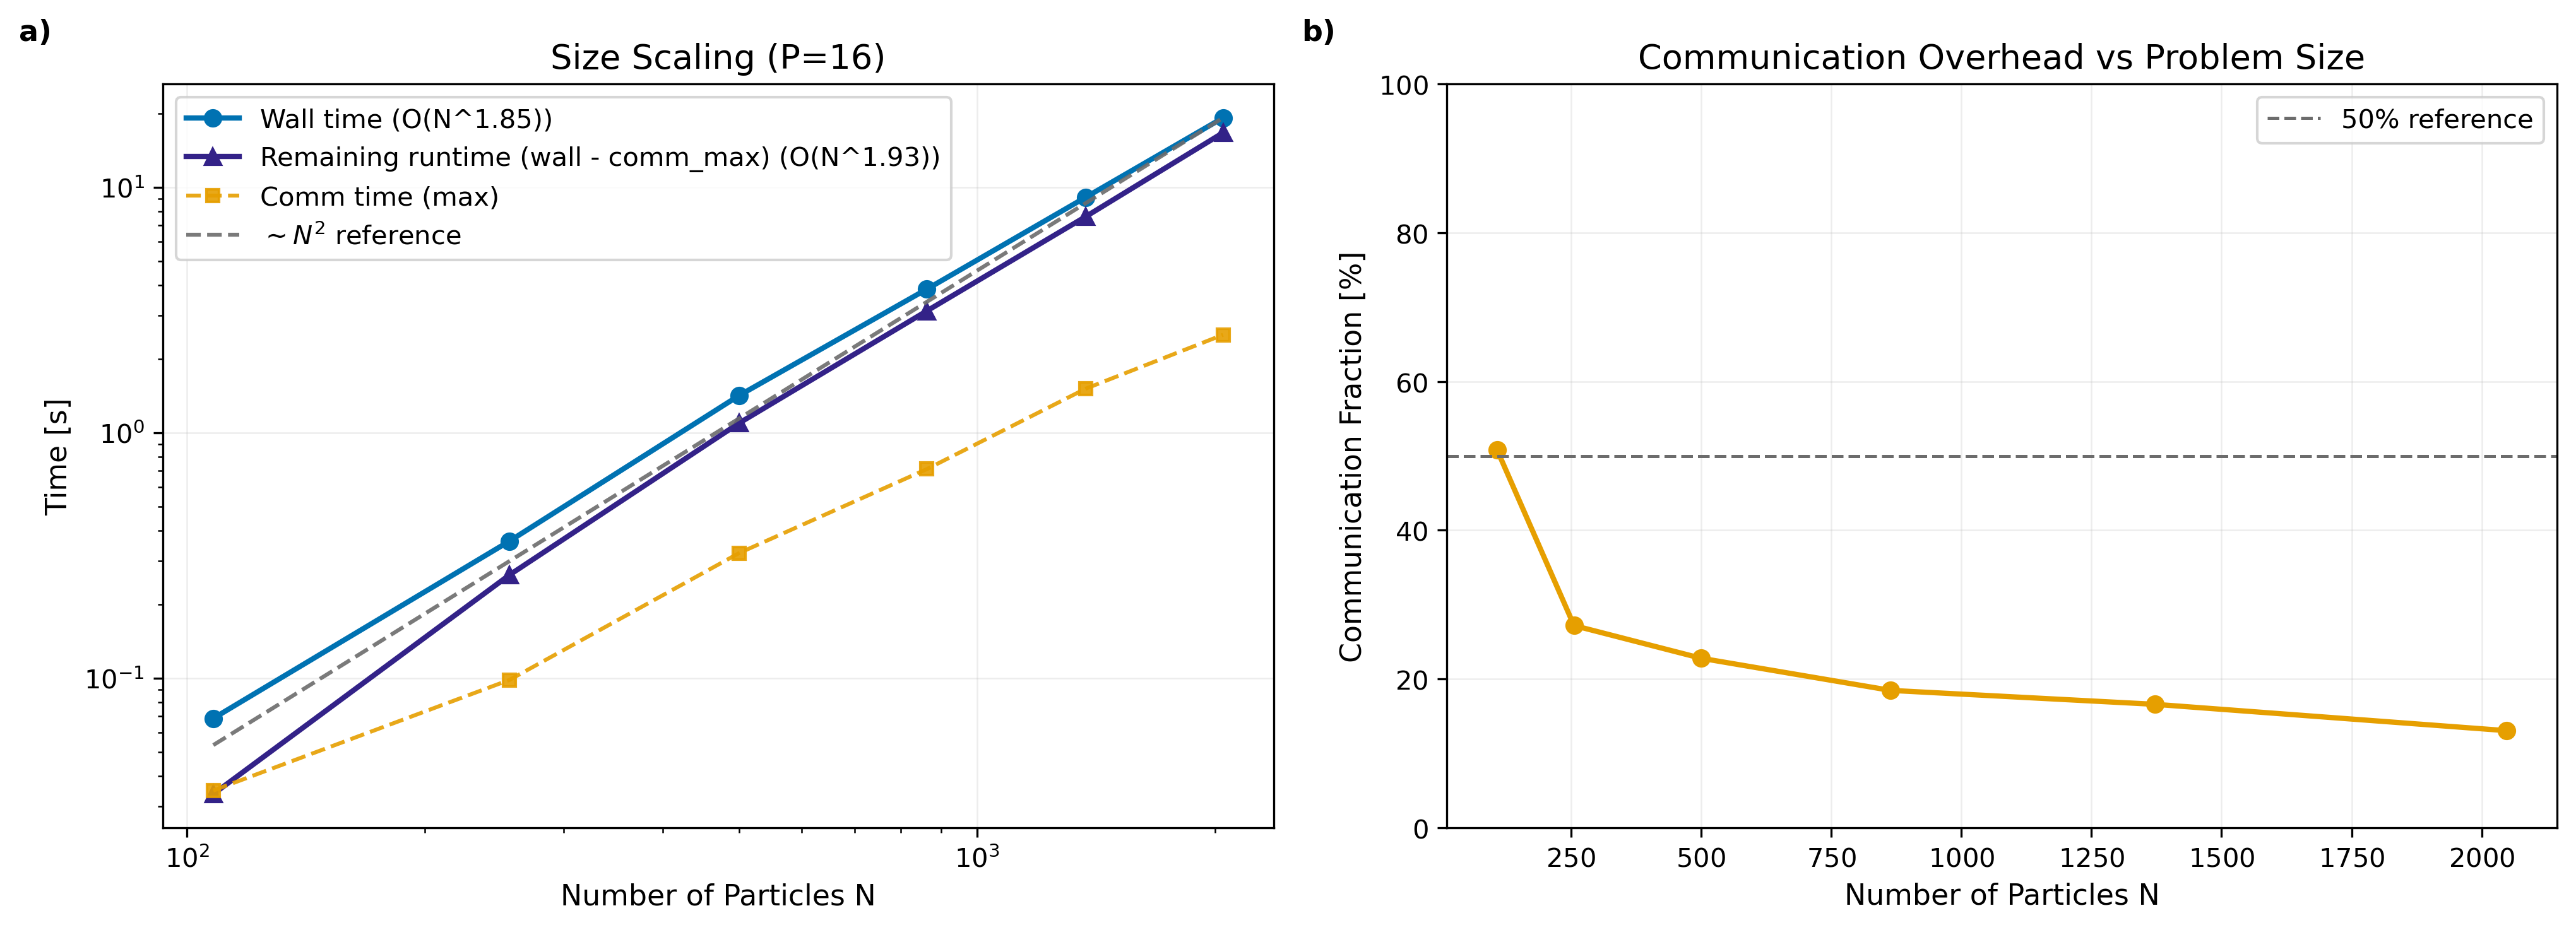
\includegraphics[width=0.96\textwidth]{results3_figure9ab_problem_size_scaling_fixed_p16.png}
  \caption{Problem-size scaling ($P=16$ fixed, Velocity-Verlet, 100 steps).
    \textbf{(a)} Log--log wall time (circles), compute-only (triangles), and
    communication (squares) vs.\ $N$, with $N^2$ reference (dash-dot).
    Empirical fits over $N\ge500$: $T_{\rm wall}\propto N^{1.85}$,
    $T_{\rm compute}\propto N^{1.93}$.
    \textbf{(b)} Communication fraction vs.\ $N$: monotone decrease from $51\%$
    ($N=108$) to $13\%$ ($N=2048$) confirms $\mathcal{O}(N^2)$ force cost
    grows faster than $\mathcal{O}(N)$ \texttt{MPI\_Allgatherv} volume.}
  \label{fig:size}
\end{figure*}

% =============================================================================
\section{Conclusions}
\label{sec:conclusions}
% =============================================================================

The harmonic oscillator tests confirm convergence orders 1.05, 2.00, 3.94
for Euler, Velocity-Verlet, and RK4, and---critically---demonstrate the
qualitative gap between symplectic and non-symplectic energy behaviour.
Velocity-Verlet's bounded oscillation at $2.5\times10^{-5}$ (in $(E-E_0)/|E_0|$)
versus Euler's monotonic $10.5\%$ drift verifies the AMM Handout's central
claim that symplecticity governs long-time stability independently of order.

For the LJ argon fluid, Velocity-Verlet conserves energy to $0.082\%$ over
the required 1~ps NVE run while Forward Euler diverges to $128\%$ with
temperature runaway to $\sim\SI{400}{K}$: Euler is conclusively unsuitable
for production MD.
RK4 achieves the highest formal accuracy (down to the IEEE~754 floor at
$3.6\times10^{-15}$) but is non-symplectic and requires four
\texttt{MPI\_Allgatherv} calls per step; it is the wrong choice for
long-time stable parallel MD.
Velocity-Verlet---one force evaluation, one collective, bounded energy---is
the correct integrator for this application.

Strong scaling achieves $S(32)=24.1\times$ at 75\% efficiency.
The Amdahl serial fraction $f\approx0.010$ captures the trend to moderate $P$,
but communication cost is the true bottleneck at high $P$: the $\mathcal{O}(N)$
\texttt{MPI\_Allgatherv} volume is independent of $P$, so communication
grows as a fraction of total time as $P$ increases.
The size-scaling exponent $N^{1.93}$ for compute-only confirms the
$\mathcal{O}(N^2)$ direct force loop as the dominant algorithmic cost.

Production-scale MD codes overcome both limitations through \emph{spatial
domain decomposition}, where each rank owns a spatial sub-domain and
communicates only halo regions with neighbouring ranks, giving
$\mathcal{O}(N^{2/3}/P)$ communication per step~\citep{AllenTildesley2017}.
Combined with Verlet or cell-list \emph{neighbour lists} to reduce force
evaluation to $\mathcal{O}(N)$, and shifted-force cutoffs to eliminate
the energy discontinuities at $r_c$, codes such as LAMMPS~\citep{Thompson2022}
and GROMACS achieve near-linear scaling to $\mathcal{O}(10^4)$ cores.
The present implementation correctly identifies the key algorithmic
trade-offs---symplecticity for stability, all-to-all communication for
simplicity, and direct pair summation for correctness---that motivate these
production-code designs.

% =============================================================================
%  REFERENCES
% =============================================================================
\bibliographystyle{plainnat}

\begin{thebibliography}{10}

\bibitem[Allen \& Tildesley(2017)]{AllenTildesley2017}
Allen M.~P., Tildesley D.~J., 2017, Computer Simulation of Liquids, 2nd edn.
Oxford University Press

\bibitem[Amdahl(1967)]{Amdahl1967}
Amdahl G.~M., 1967, Proc.\ AFIPS Spring Joint Comput.\ Conf., pp. 483--485

\bibitem[{Cambridge MPhil}(2025)]{AMMHandout}
{Cambridge MPhil Scientific Computing}, 2025, Atomistic Modelling of Materials:
Lecture Handout. Course material

\bibitem[Frenkel \& Smit(2002)]{FrenkelSmit2002}
Frenkel D., Smit B., 2002, Understanding Molecular Simulation, 2nd edn.
Academic Press

\bibitem[Rahman(1964)]{Rahman1964}
Rahman A., 1964, Phys.\ Rev., 136, A405

\bibitem[Swope et~al.(1982)]{Swope1982}
Swope W.~C., Andersen H.~C., Berens P.~H., Wilson K.~R., 1982,
J.\ Chem.\ Phys., 76, 637

\bibitem[Thompson et~al.(2022)]{Thompson2022}
Thompson A.~P. et~al., 2022, Comput.\ Phys.\ Commun., 271, 108171

\bibitem[Verlet(1967)]{Verlet1967}
Verlet L., 1967, Phys.\ Rev., 159, 98

\end{thebibliography}

\end{document}